\documentclass[runningheads, draft]{llncs}
%\documentclass{llncs}
%\documentclass{article}

% !TeX root = main.tex

\usepackage[T1]{fontenc}
\usepackage[margin=1in]{geometry}
\usepackage{graphicx}
\usepackage{authblk}
%S\usepackage[ruled,vlined]{algorithm2e}

\usepackage{float}

\usepackage[english]{babel}
\usepackage[utf8]{inputenc}

\usepackage{hyperref}
\hypersetup{final}

\usepackage{footmisc} %footnotes handling

\usepackage{amsmath, amssymb, mathtools}
\usepackage{listings}
\usepackage{graphicx, color, xcolor}
\usepackage{xspace} %list of punctuation marks 
\usepackage{enumitem}
\usepackage{multirow}
\usepackage{ifdraft}
%\usepackage{draftwatermark}

\usepackage{setspace}

\usepackage{mdframed} % frame figures

%\ifdraft{
%	% \usepackage[color = {[rgb]{0.9, 0.9, 0.9}}]{draftwatermark}
%	\usepackage{draftwatermark}
%	\SetWatermarkText{Draft}
%	\SetWatermarkScale{4}
%}

\ifdraft{\usepackage[colorinlistoftodos, textwidth = 40mm]{todonotes}}
{\usepackage[disable, colorinlistoftodos, textwidth = 40mm]{todonotes}}

\usepackage{tikz,tikz-cd}
% !TeX root = main.tex

% Doc sytle
\setcounter{secnumdepth}{3} %enumerate sections up to depth 3 (subsubsection)
% Set the first-level itemize label to use math mode \bullet
\setlist[itemize,1]{label=$\bullet$}

% Working directory
\newcommand{\definedir}[2]{\newcommand{#1}{#2}}
\definedir{\secs}{../sections}
\definedir{\figs}{../figures}
\definedir{\bib}{../bibliography}

% Comments
\newcommand{\marta}[1]{\todo[size=\small, color=red!40]{\textbf{Marta}: #1}}
\newcommand{\martai}[1]{\todo[inline, size=\small, color=red!40]{\textbf{Marta}: #1}}
\newcommand{\pau}[1]{\todo[size=\small, color=blue!40]{\textbf{Pau}: #1}}
\newcommand{\paui}[1]{\todo[inline, size=\small, color=blue!40]{\textbf{Pau}: #1}}
\newcommand{\jordi}[1]{\todo[size=\small, color=green!40]{\textbf{Jordi}: #1}}
\newcommand{\jordii}[1]{\todo[inline, size=\small, color=green!40]{\textbf{Jordi}: #1}}

% Freefootnote
\let\svthefootnote\thefootnote
\newcommand\freefootnote[1]{%
	\let\thefootnote\relax%
	\footnotetext{#1}%
	\let\thefootnote\svthefootnote%
}

% Table of contents style
% Make section entries bold in ToC
\makeatletter
\renewcommand{\@dotsep}{4.5}
\renewcommand{\l@section}[2]{\addpenalty{\@secpenalty}
	\addvspace{1.0em plus 1pt}
	\@tempdima=1.5em
	\parindent \z@ \rightskip \@pnumwidth
	\parfillskip -\@pnumwidth
	{\leavevmode
		\advance\leftskip\@tempdima
		\hskip -\leftskip
		\bfseries #1\hfil \hbox to\@pnumwidth{\hss #2}}\par}
\makeatother

% Colours
\definecolor{cred}{rgb}{1, 0.5, 0.5}
\definecolor{cgreen}{rgb}{0.5, 1, 0.5}
\definecolor{cblue}{rgb}{0.5, 0.5, 1}

% Hyperref setup
%\hypersetup{
%	final=true,
%	colorlinks=true,
%	linkcolor=cblue,
%	urlcolor=black,
%	citecolor=cblue,
%}

% Mathbb
\newcommand{\N}{\ensuremath{\mathbb{N}}\xspace}
\newcommand{\Z}{\ensuremath{\mathbb{Z}}\xspace}
\newcommand{\G}{\ensuremath{\mathbb{G}}\xspace}
\newcommand{\F}{\ensuremath{\mathbb{F}}\xspace}
\newcommand{\J}{\ensuremath{\mathbb{J}}\xspace}

% Elliptic curves
\newcommand{\BW}[1]{\ensuremath{{#1}^{\text{\tiny \sf BW}}}\xspace}
\newcommand{\BLS}[1]{\ensuremath{{#1}^{\text{\tiny \sf BLS}}}\xspace}
\newcommand{\BN}[1]{\ensuremath{{#1}^{\text{\tiny \sf BN}}}\xspace}
\newcommand{\BJ}[1]{\ensuremath{{#1}^{\text{\tiny \sf BJ}}}\xspace}
\newcommand{\SEC}[1]{\ensuremath{{#1}^{\text{\tiny \sf SEC}}}\xspace}

% Circuits
\newcommand{\public}{{\sf\color{teal}public}\xspace}
\newcommand{\private}{{\sf\color{red}private}\xspace}

% Ballot protocol
\newcommand{\ballotstyle}[1]{\texttt{#1}\xspace}
\newcommand{\maxcount}{\ballotstyle{maxCount}}
\newcommand{\maxvalue}{\ballotstyle{maxValue}}
\newcommand{\minvalue}{\ballotstyle{minValue}}
\newcommand{\uniquevalues}{\ballotstyle{uniqueValues}}
\newcommand{\maxtotalcost}{\ballotstyle{maxTotalCost}}
\newcommand{\mintotalcost}{\ballotstyle{minTotalCost}}
\newcommand{\costexponent}{\ballotstyle{costExponent}}

% Voting protocol
\newcommand{\variablestyle}[1]{\texttt{#1}\xspace}
\newcommand{\voteproof}{\variablestyle{voteProof}}
\newcommand{\censusproof}{\variablestyle{censusProof}}
\newcommand{\authenticationproof}{\variablestyle{authenticationProof}}
\newcommand{\voteid}{\variablestyle{voteID}}
\newcommand{\ballot}{\variablestyle{ballot}}
\newcommand{\vote}{\variablestyle{vote}}
\newcommand{\processid}{\variablestyle{processID}}
\newcommand{\censuspf}{\variablestyle{censusProof}}
\newcommand{\commitment}{\variablestyle{identityCommitment}}
\newcommand{\nullifier}{\variablestyle{nullifier}}
\newcommand{\encryptedballot}{\variablestyle{encryptedBallot}}
\newcommand{\zkproof}{\variablestyle{ZKproof}}
\newcommand{\signature}{\variablestyle{signature}}
\newcommand{\address}{\variablestyle{address}}

% State Merkle tree
\newcommand{\censusroot}{\variablestyle{censusRoot}}
\newcommand{\type}{\variablestyle{type}}
\newcommand{\ballotmode}{\variablestyle{ballotMode}}
\newcommand{\epk}{\variablestyle{encryptionKey}}
\newcommand{\addaccumulator}{\variablestyle{addedResultsAccumulator}}
\newcommand{\substractaccumulator}{\variablestyle{substractResultsAccumulator}}
\newcommand{\addresses}{\variablestyle{addresses}}
\newcommand{\nullifiers}{\variablestyle{nullifiers}}
\newcommand{\weight}{\variablestyle{weight}}

% Others
\newcommand{\noi}{\noindent}
\newcommand{\conc}{\:||\:}

% Hyperlinks
\newcommand{\hlset}[1]{\hypertarget{\detokenize{#1}}{#1}}
\newcommand{\hlget}[1]{\hyperlink{\detokenize{#1}}{#1}}

% Cryptographic primitives
\newcommand{\methodstyle}[1]{{\sf{#1}}\xspace}
\newcommand{\Keccak}{\methodstyle{Hash_1}}
\newcommand{\Poseidon}{\methodstyle{Hash_2}}
\newcommand{\Mimc}{\methodstyle{Hash_3}}
\newcommand{\Enc}{\methodstyle{Enc}}
\newcommand{\Dec}{\methodstyle{Dec}}
\newcommand{\EncAdd}{\methodstyle{EncAdd}}
\newcommand{\ReEnc}{\methodstyle{ReEnc}}
\newcommand{\SSign}{\methodstyle{S.Sign}}
\newcommand{\SVer}{\methodstyle{S.Verify}}
\newcommand{\GenerateShares}{\methodstyle{GenerateShares}}
\newcommand{\VerifyShare}{\methodstyle{VerifyShare}}
\newcommand{\DerivePublicKey}{\methodstyle{DerivePublicKey}}
\newcommand{\DeriveSecretShare}{\methodstyle{DeriveSecretShare}}

\newcommand{\blinder}[1][]{{\sf{blinder}^{#1}}}
\newcommand{\pk}[1][]{{\sf{pk}^{#1}}}
\newcommand{\sk}[1][]{{\sf{sk}^{#1}}} 
\newcommand{\msg}[1][]{{\sf{message}^{#1}}}
\newcommand{\enc}[1][]{{\sf{ciphertext}^{#1}}}
\newcommand{\sample}{\xleftarrow{\$}}

% VOC token
\newcommand{\token}{VOC\xspace}
\newcommand{\vocstyle}[1]{{\sf{#1}}\xspace}
\newcommand{\baseCost}{\vocstyle{baseCost}}
\newcommand{\capacityCost}{\vocstyle{capacityCost}}
\newcommand{\durationCost}{\vocstyle{durationCost}}
\newcommand{\fixedCost}{\vocstyle{fixedCost}}
\newcommand{\maxVotes}{\vocstyle{maxVotes}}
\newcommand{\maxDuration}{\vocstyle{maxDuration}}
\newcommand{\numSequencers}{\vocstyle{numSequencers}}
\newcommand{\processDuration}{\vocstyle{processDuration}}
\newcommand{\reimbursement}{\vocstyle{reimbursement}}
\newcommand{\securityCost}{\vocstyle{securityCost}}
\newcommand{\sequencerReward}{\vocstyle{sequencerReward}}
\newcommand{\slashedAmount}{\vocstyle{slashedAmount}}
\newcommand{\stakedCollateral}{\vocstyle{stakedCollateral}}
\newcommand{\totalCost}{\vocstyle{totalCost}}
\newcommand{\totalReward}{\vocstyle{totalReward}}
\newcommand{\totalRewrites}{\vocstyle{totalRewrites}}
\newcommand{\totalSequencers}{\vocstyle{totalSequencers}}
\newcommand{\totalVotingProcesses}{\vocstyle{totalVotingProcesses}}
\newcommand{\usedSequencers}{\vocstyle{usedSequencers}}
\newcommand{\votes}{\vocstyle{votes}}
\newcommand{\voteRewrites}{\vocstyle{voteRewrites}}

% Misc
\newcommand{\davinci}{DAVINCI\xspace}
\newcommand{\Davinci}{DAVINCI\xspace}

% Draft watermark
%\ifdraft{\SetWatermarkScale{4}}{\SetWatermarkScale{0}}

% New foonote referencing a previous footmark
\makeatletter
\newcommand\footnoteref[1]{\protected@xdef\@thefnmark{\ref{#1}}\@footnotemark}
\makeatother

\title{\textsc{DAVINCI}\vspace{-0.4cm}}
%Decentralized autonomous vote integrity network with cryptographic inference
\author{Authors: Pau Escrich and Jordi Piñana from Vocdoni Association}
\institute{Last update: \today}

% election, vote, polling, ballot, selection, decision-making process

\begin{document}
	
\maketitle

%enumerate pages
\pagestyle{plain}
\thispagestyle{plain}

\addcontentsline{toc}{section}{\protect\numberline{}Abstract}
\begin{abstract}
		\Davinci is the evolution of the Vocdoni voting protocol, designed to empower civil society by providing essential tools for secure, verifiable, and anonymous digital voting. Leveraging recent advancements in zero-knowledge (ZK) proof systems and blockchain technology, \davinci transitions to a specialized ZK-rollup system that inherits network security from settlement layers like Ethereum mainnet. The system relies on cryptographic proofs to ensure integrity and security, eliminating the need for centralized authorities. By integrating ZK-SNARKs and threshold homomorphic encryption, \davinci enables end-to-end verifiability, privacy, and trustlessness in the voting process. The protocol employs a distributed key generation among sequencers, coordinated via Ethereum smart contracts, and utilizes Ethereum data blobs for data availability. With a focus on accessibility, scalability, receipt-freeness, and automation, \davinci aims to facilitate high-frequency, low-cost voting, fostering mass adoption of e-voting and simplifying civil participation. Finally, the introduction of the Vocdoni token (\token) aligns incentives among participants, ensuring the system's sustainability and enabling decentralized governance.
		
		Moreover, the design of \davinci is grounded in practicality; all components have been implemented using current technologies and have undergone proof-of-concept testing. This ensures that the proposed architecture is not merely theoretical but a viable solution ready for short-term deployment.
		
%	    \freefootnote{\scriptsize{Authors are listed in alphabetical order (\url{https://www.ams.org/profession/leaders/CultureStatement04.pdf}).}}
\end{abstract}

\martai{Change Vocdoni to DAVINCI.}

\martai{Mention that the spec can be tailored to the needs of the specific vote. So, here we present some default configuration, but some of the pieces can be changed (specially the cryptographic schemes or curves). For this reason, we tried to make this document modular (like the code), to facilitate the changes and the analysis of the consequences.}

\martai{Separate the roles of the sequencers from key generators?}

\setcounter{tocdepth}{3}
\makeatletter
\renewcommand*\l@author[2]{}
\renewcommand*\l@title[2]{}
\makeatletter
\tableofcontents

%\pagebreak
\section*{Vocdoni}
\addcontentsline{toc}{section}{\protect\numberline{}Vocdoni}
\label{sec:intro-old}
% !TeX root = ../build/main.tex

\paragraph{Vision and background.}

Voĉdoni, meaning “to give voice” in Esperanto, embodies our mission to empower civil society from the grassroots level. We aim to build essential primitives and tools that enable any collective—from small groups to millions of citizens—to be heard, regardless of their circumstances or available resources. Our philosophy envisions voting beyond traditional nation-state elections; we see it as a collective signaling mechanism with cryptographic guarantees of integrity and outcome. To address the challenge, we developed a end-to-end verifiable and anonymous voting system designed to work on any device, including smartphones. We also successfuly deployed an infrastructure that maximizes resilience, neutrality, and transparency.

In 2018, when Vocdoni began, zkSNARKs was just an emerging technology. We chose to base our solution on a customized Byzantine fault tolerant layer-1 (L1) blockchain called Vochain. This allowed us to achieve scalability (approximately 700 transactions per second), to leverage advanced cryptographic tools that are prohibitively expensive on EVM-based blockchains, and enable users to send voting transactions without costs. This experience has provided us with invaluable insights that have enabled us to overcome technical and operational challenges. Although this solution has effectively met user requirements and demonstrated its viability, further development is essential for its widespread adoption as a universal voting protocol.

\Davinci represents the evolution of the Vocdoni voting protocol. It integrates smart contracts for orchestration, a zkSNARK-based state machine for verifying and accumulating votes, and a decentralized data availability layer to ensure censorship resistance.

\paragraph{Design principles.}

To build the \davinci stack, we adhere to the following design principles:

\begin{enumerate}
	\item \textbf{Cryptography as the source of truth}: we rely exclusively on cryptographic proofs to ensure the integrity and security of the voting process. By trusting only in cryptography, we eliminate the need for centralized authorities, making the system inherently secure and transparent.
	
	\item \textbf{Trustlessness}: our system operates without requiring trust in any single party. Through cryptographic protocols and decentralized infrastructure, we ensure system integrity and prevent compromise from any malicious actor.
	
	\item \textbf{End-to-end verifiability}: every voter can verify their ballot from casting to result computation (individual verifiability). Additionally, any third party can audit the election data to confirm results (universal verifiability) and verify that each vote comes from a uniquely registered voter (eligibility verifiability). Transparent cryptographic mechanisms make this possible.
	
	\item \textbf{Composability}: the system is modular, consisting of interchangeable components that can be rearranged or integrated with external systems via adaptable interfaces. This allows for redundancy, flexibility, and seamless integration with third-party applications, exemplified by our voting-as-a-service APIs.
	
	\item \textbf{Accessibility}: Vocdoni’s voting platform (App) is open source, universally available and user-friendly. The interface is intuitive for all users, including those less familiar with technology, and accommodates voters that use assistive technologies like screen readers.
	
	\item \textbf{Open source}: by releasing our code openly, we invite anyone to audit and contribute, enhancing security and fostering community engagement. Transparency prevents security through obscurity and accelerates innovation.
	
	\item \textbf{Resilience}: we design for robustness against hardware failures, network outages, and censorship. Infrastructure decentralization and distributed ownership enhance system availability and resistance to attacks.
	
	\item \textbf{Scalability}: our solution processes votes at high throughput, exceeding current requirements to accommodate future growth. The decentralized infrastructure scales organically as usage increases, ensuring consistent performance.
	
	\item \textbf{Receipt-freeness}: to mitigate risks of collusion, coercion, and vote-buying, the system enables voters to verify their votes without being able to prove to others how they voted, thus reducing incentives for coercion and bribery. Additionally, voters are allowed to overwrite their votes while maintaining secrecy.
	
	\item \textbf{Automation}: we minimize human intervention through smart contracts and cryptographic protocols, reducing costs and human error. Automation ensures consistent operation and frees resources for voter support and auditing.
\end{enumerate}

\paragraph{Components overview.}

Below, we detail the components of the architecture that collectively support the operation and management of the voting system.

\begin{figure}[h]
	\centerline{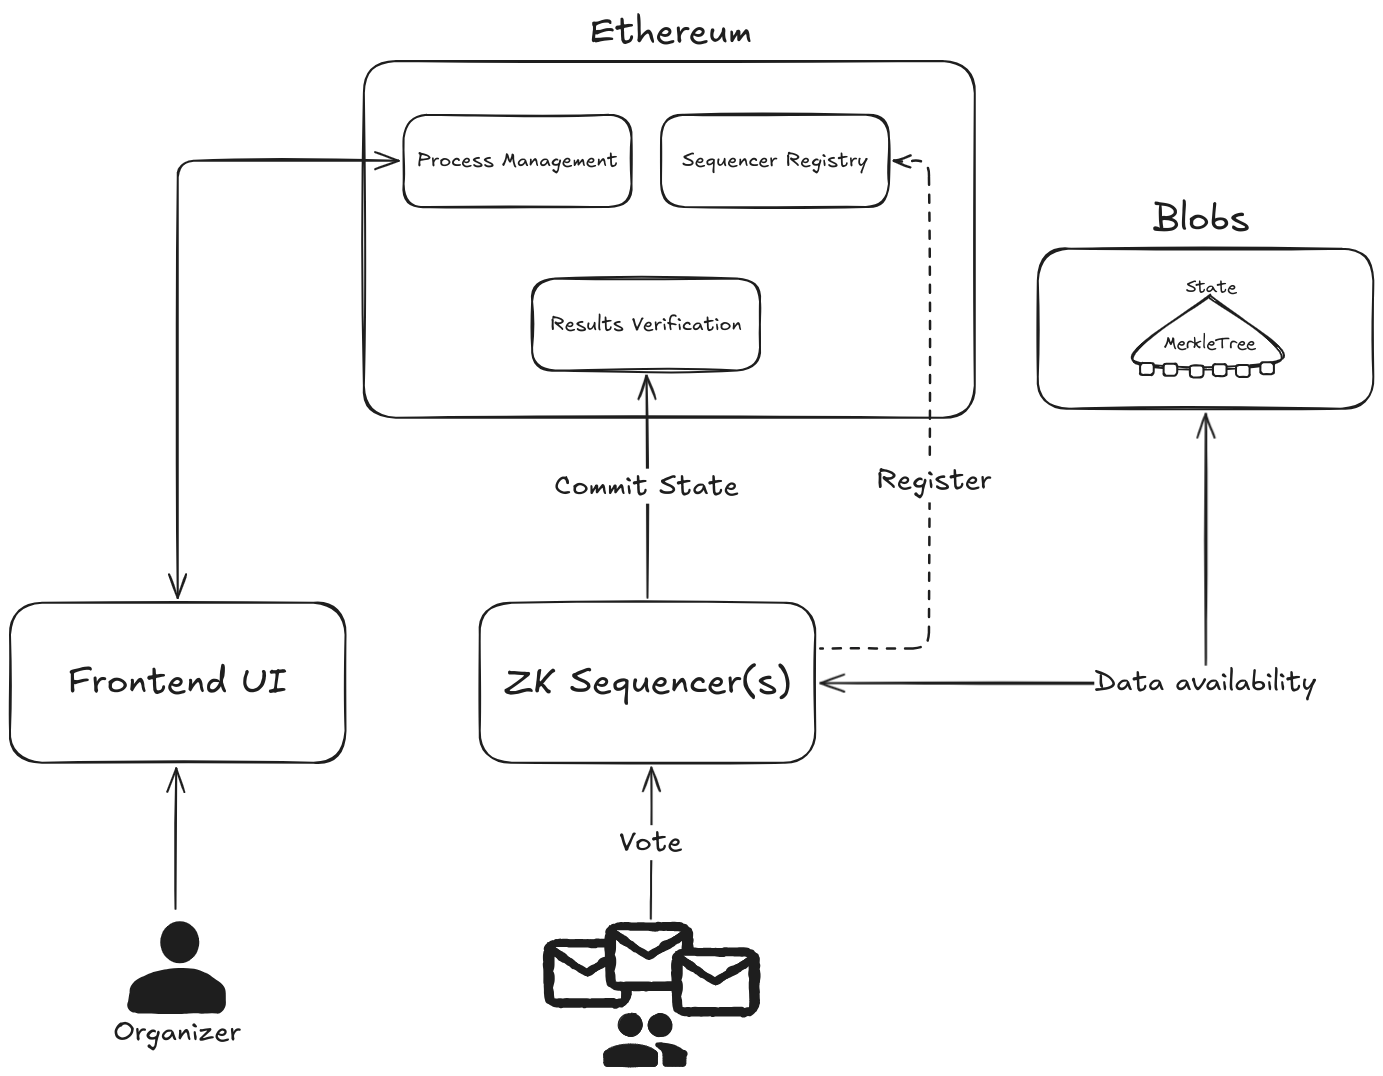
\includegraphics[width=400pt,draft=false]{\figs/architecture.png}}
	\caption{Caption.}
	\label{fig:circuit-inputs}
\end{figure}

\begin{enumerate}
	\item \textbf{Ethereum}. An Ethereum compatible network is used as the source of truth for the voting system. By leveraging an EVM blockchain, the process management ensures that all transitions are immutable and verifiable by all participants. To this end, we implement several smart contracts.
		\begin{itemize}
			\item \textbf{Process management}: Responsible for the lifecycle management of voting processes. It includes the initiation, monitoring, execution, and closure of voting events.
			\item \textbf{Results verification}: For each voting process, this smart contract maintains the integrity of the cast votes and process lifecycle. It verifies that each state transition committed by a ZK sequencer adheres to the predefined rules.			
			\item \textbf{Sequencer registry}: This smart contract keeps track of the existing available sequencers, stores the collateral to ensure good behavior, and it's used to coordinate the distributed key generation when a new Process is created.
		\end{itemize}
	\item \textbf{Sequencer}. The Sequencer is a specialized component designed to handle the voting process using zero-knowledge proof mechanisms. It ensures that all transactions related to this process are validated and sequenced. The Sequencers periodically commit the state of the voting process to Ethereum.
	\item \textbf{Frontend user interface}. The user interface serves as the primary interaction layer for voters and organizers. It provides tools and functionalities needed by organizers to set up, manage, and oversee elections. This interface simplifies the complexities involved in managing a decentralized vote.
	\item \textbf{Data availability}. For each voting process, the system needs to keep track of the current State Merkle Tree, which contains all information of such processes. A public data availability layer, ensures that all state transitions are available and verifiable and allows the participation of multiple sequencers within the same voting process.
\end{enumerate}


\section{Introduction}
\label{sec:intro}
% !TeX root = ../build/main.tex

Online voting remains one of the most studied yet elusive applications in applied cryptography. As digital services expand across both public and private sectors, secure and universally verifiable online voting systems have become an increasingly desirable goal. Remote electronic voting promises scalability, accessibility, and administrative efficiency; yet the design of systems that simultaneously ensure privacy, integrity, coercion resistance, and transparency under realistic adversarial models remains a formidable challenge. Numerous deployments—including iVote, Helios, and the Estonian I‑voting system—have revealed deep-rooted usability flaws and security gaps, particularly when verifiability mechanisms are either poorly understood by users or reliant on centralized infrastructure.

Against this backdrop, the Vocdoni project was initiated in 2018 with the aim of rethinking online voting from first principles. The name Voĉdoni, meaning “to give voice” in Esperanto, reflects the project’s foundational goal: to empower collectives—from small associations to millions of citizens—to engage in secure and verifiable decision-making, regardless of technological or institutional barriers. Central to this vision was the idea that voting is not limited to formal governmental elections but serves as a more general-purpose mechanism for collective signaling. Vocdoni introduced a fully anonymous, end-to-end verifiable voting system designed to operate efficiently across a range of devices, including smartphones. To support these goals, the team deployed a custom infrastructure emphasizing resilience, neutrality, and transparency.

Technically, the architecture of Vocdoni was grounded on a bespoke Byzantine Fault Tolerant (BFT) layer-1 blockchain, named Vochain. At the time, zero-knowledge proof systems such as zkSNARKs were emerging but not yet practical for most deployments. Vochain provided a performant and low-cost environment (achieving approximately 700 transactions per second) where advanced cryptographic tools could be used without the constraints imposed by EVM-based blockchains. The ability to issue voting transactions without requiring user fees enabled broader accessibility. Over several years of development and deployment, this architecture proved both viable and valuable in practice. However, broader adoption as a universal voting protocol highlighted the need for further architectural refinements and stronger formal guarantees.

In this work, we introduce \davinci, a new protocol that builds upon the lessons and conceptual groundwork laid by Vocdoni. DaVinci adopts a modular design and integrates state-of-the-art cryptographic tools—including succinct zero-knowledge proofs, improved bulletin board constructions, and robust coercion resistance mechanisms—reflecting the most recent advances in academic research. Unlike monolithic designs, DaVinci is conceived as a composable primitive: a foundational layer intended to support secure and verifiable voting in diverse contexts, from blockchain governance to institutional elections. This shift in design philosophy aims to address long-standing challenges in the field, offering a cleaner abstraction with clearer security boundaries and formal underpinnings.

\subsection{Contributions}
\label{sec:introduction:contributions}

\begin{itemize}
	\item The Vocdoni voting protocol.
	\item The Vocdoni ballot protocol.
\end{itemize}

\subsection{Related work}
\label{sec:introduction:sota}

\begin{itemize}
	\item State of the art of e-voting: \url{https://azkr.org/blog/evoting-review/}.
\end{itemize}

\subsection{Paper organization}
\label{sec:introduction:organization}

\begin{itemize}
	\item Section~\ref{sec:background}: background.
	\item Section~\ref{sec:protocol-intuition}: high overview of the election process. We omit technical details.
	\item Section~\ref{sec:cryptographic-primitives}: cryptographic primitives used in the voting process. A description of the primitives but also the details of their instantiation, that is, the specific protocols being used.
	\item Section~\ref{sec:vocdoni-protocol}: description of the voting process.
	\item Section~\ref{sec:ballot-protocol}: a proposed protocol for ballots. The rules of this protocol are implemented in the process management smart contracts.
	\item Section~\ref{sec:token}: the Vocdoni token.
	\item Section~\ref{sec:analysis}: analysis of the proposed protocols. It includes a security discussion of the properties of the protocol, implementation details, and a performance evaluation.
	\item Section~\ref{sec:conclusions}: we finish with some last remarks.
\end{itemize}

\section{Background}
\label{sec:background}
% !TeX root = ../build/main.tex

\subsection{Interplanetary file system (IPFS)}
\label{sec:background:ipfs}

\begin{itemize}
	\item Brief introduction to IPFS.
\end{itemize}

\subsection{Ethereum}
\label{sec:background:ethereum}

\begin{itemize}
	\item Ethereum blockchain (say transactions have a cost fee).
	\item Ethereum smart contracts.
	
	\textit{Old text: Ethereum smart contracts are employed to orchestrate the voting process, manage state transitions, and store critical data, such as the current state root and encryption public keys. These smart contracts provide a trustless environment, ensuring that all participants can be confident that the voting process rules are correctly enforced.}
	
	\item Ethereum data blobs.
	
	\textit{Old text: EIP-4844 is used for data availability, enabling the storage of state transition data in the form of Ethereum data blobs. This mechanism allows sequencers to collaborate on the construction and verification of the voting process state, ensuring efficient and decentralized data availability.}
	
\end{itemize}

\subsection{Zero-knowledge proofs}
\label{sec:background:zkp}

\begin{itemize}
	\item Introduce ZK-SNARKs.
	\item Introduce arithmetic circuits (arithmetic circuit satisfiability).
\end{itemize}

\section{Protocol intuition}
\label{sec:protocol-intuition}
% !TeX root = ../build/main.tex

All the voting process is governed by the rules encoded in three smart contracts: the \textit{process management}, the \textit{sequencer registry}, and the \textit{results verification} smart contract. All these three contracts are deployed on the Ethereum blockchain, and ensure that the execution of all steps is transparent and unalterable. The protocol consists of 5 phases, as illustrated in Figure~\ref{fig:protocol-intuition}, and described below.\\

\begin{figure}[h]	
	\centerline{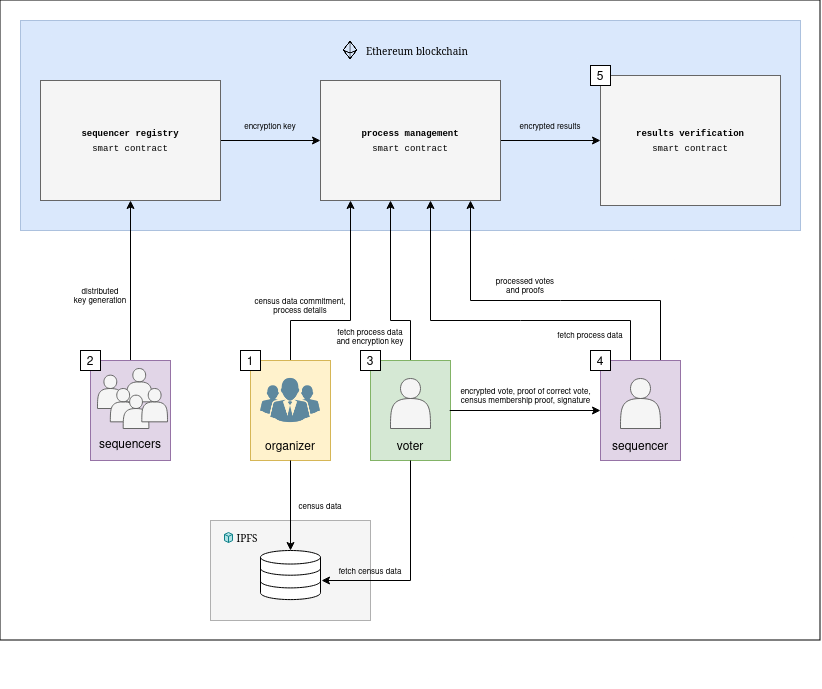
\includegraphics[width=350pt,draft=false]{\figs/protocol-intuition-flow}}
	\caption{Overview of the protocol flow.}
	\label{fig:protocol-intuition}
\end{figure}

\paragraph{$\boxed{1}$ Voting setup.}

In the first phase, the organizing entity gathers all census data and generates a cryptographic commitment to this data. %using a Merkle tree (MT) root. 
Additionally, the organizer defines the voting parameters, including the number of voting options and the vote-counting mechanism (e.g., weighted voting, quadratic voting, etc.). Once these details are set, the organizer submits a transaction to the process management smart contract on the Ethereum blockchain. This transaction publicly records the voting parameters and census commitment, ensuring transparency and preventing any subsequent alterations to the voting setup.

\paragraph{$\boxed{2}$ Encryption key generation.}

A designated group of participants, referred to as \textit{sequencers}, collaboratively generate a shared encryption public key, which voters will use to encrypt their votes. This key is established through a distributed key generation (DKG) protocol, ensuring that no single party can control or reconstruct the corresponding private key independently. 
Sequencers have a dual role in the protocol. In addition to generating the encryption key, they are also responsible for collecting votes from voters during the election. Consequently, their public key and the necessary information to contact them off-chain must be registered in the sequencer registry smart contract. Once the encryption public key is securely computed and published in the sequencer registry smart contract, the voting phase can start.

\paragraph{$\boxed{3}$ Voting.}

Voters select their preferred option according to the voting rules established by the organizer and captured in the process management smart contract. Instead of submitting their votes directly on-chain, they send them off-chain to a sequencer of their choice for processing. To ensure privacy, votes are encrypted using the available encryption public key. 
Additionally, users compute a unique vote identifier that will allow them to verify that their vote has been included in the final result. Alongside the encrypted vote and the vote identifier, each voter must also provide the following data: a proof of valid voting, demonstrating that the vote complies with the election rules; a proof of eligibility, verifying that they are registered in the census; and a proof of identity ownership, in the form of a digital signature, confirming that they are the legitimate voter and are not impersonating someone else. Finally, to mitigate coercion and vote-buying, the protocol allows voters to overwrite their vote any number of times during the voting phase. 

\paragraph{$\boxed{4}$ Votes collection.}

During this phase, sequencers collect encrypted votes from multiple voters along with their corresponding proofs, and verify the validity of these submissions. That is, sequencers
verify the signatures, to ensure the votes were cast by legitimate voters, they verify the proof of compliance, confirming that each vote adheres to the polling rules, and the census membership proofs against the commitment to the census data that was originally registered in the process management smart contract. Once the sequencers have processed and verified all votes, they must prove that these verifications were performed correctly. Instead of submitting individual verifications for each vote, they generate a single zero-knowledge (ZK) proof that attests to the correctness of all verifications.
%they compress multiple individual verification into one.
Additionally, the sequencers reencrypt the votes and generate a proof of the correct reencryption computation. While this process does not alter the final tally, it prevents voters from decrypting their original vote. This step mitigates vote selling or coercion, as voters are no longer able to prove their choice to third parties. Finally, the sequencers submit the reencrypted votes along with their verification and reencryption proofs to the process management smart contract. The smart contract verifies all the proofs provided by the sequencers to check that they complied with the protocol.

\paragraph{$\boxed{5}$ Results verification.}
\textit{At the conclusion of the voting period, the smart contract ceases to accept new state updates, effectively finalizing the process. The final state is then available on-chain for verification, providing an immutable record of the voting outcome.}
\marta{I did not look into the results decryption/verification part yet. A short description should be given here.}

\section{Cryptographic primitives} %building blocks
\label{sec:cryptographic-primitives}
% !TeX root = ../build/main.tex

In this section, we detail the cryptographic primitives used in Section~\ref{sec:vocdoni-protocol}. We briefly introduce elliptic curves, hash functions, Merkle trees, encryption schemes, and proof systems used in the protocol. We also specify at each step the concrete parameters with which each of the primitives is instantiated.\\

\martai{Maybe it should go under the protocol section?}

%\paragraph{Notation.} Throughout the document, we use the following conventions. Given a set $S$, we denote sampling an element $x$ uniformly at random from $S$ by $x \sample S$. We denote all bitstrings of arbitrary length by $\{0,1\}^*$. 
%Any group $\G$ used is of a large prime order, and we assume that the discrete logarithm problem is hard in $\G$. If two elements are denoted by the same letter in upper and lower case, e.g. $a, A$, this often means that $A$ is a public key corresponding to the secret key $a$. 
%$\F_p$ denotes de finite field of order $p$, and $\F_p^* = \F_p/\{0\}$.

\subsection{Elliptic curves}
\label{sec:cryptographic-primitives:elliptic-curves}

\Davinci relies on multiple elliptic curves to ensure interoperability with Ethereum, compatibility with available cryptographic primitives, and efficient in-circuit operations. On the one hand, SECP256K1~\cite{brown10sec} is used because Ethereum public keys are elements of this curve. As \Davinci assumes each voter holds a standard Ethereum address, cryptographic operations such as digital signatures and identity verification rely on SECP256K1 to match the Ethereum ecosystem. On the other hand, BN254~\cite{jancar20bn256} is chosen because it is the curve supported by Ethereum's precompiled contracts for zero-knowledge proof verification, which makes it ideal for verifying SNARK proofs on-chain with minimal gas cost. then, BabyJubjub~\cite{belles21twisted} is used as an inner curve for elliptic curve operations within arithmetic circuits. Finally, BLS12-377~\cite{bowe20zexe} and BW6-761~\cite{elhousni20optimized} are used to enable recursive proof composition. More specifically, BLS12-377 acts as the inner curve for constructing proofs, while BW6-761 serves as the outer curve that verifies those proofs within larger zkSNARK circuits. This pairing enables succinct verification and composability of zkSNARKs within other zkSNARKs, which we use for \davinci’s aggregation and state transition logic. Below, we give the details of these curves.

\paragraph{Parameters.}

\begin{itemize}
	%
	\item[$\bullet$] $p = \tt{\hspace{0.04cm}0xfffffffffffffffffffffffffffffffffffffffffffffffffffffffefffffc2f}$ (256-bit prime).
	\item[$\bullet$] $q = \tt{\hspace{0.01cm}0xfffffffffffffffffffffffffffffffebaaedce6af48a03bbfd25e8cd0364141}$ (256-bit prime).	
	%
	\item[$\bullet$] $r = \tt{0x2523648240000001ba344d80000000086121000000000013a700000000000013}$ (254-bit prime).
	\item[$\bullet$] $s = \tt{\hspace{0.04cm}0x2523648240000001ba344d8000000007ff9f800000000010a10000000000000d}$ (254-bit prime).
	\item[$\bullet$] $t = \tt{\hspace{0.01cm}0x60c89ce5c263405370a08b6d0302b0bab3eedb83920ee0a677297dc392126f1}$ (251-bit prime).
	%
	\item[$\bullet$] $u = \tt{0x122e824fb83ce0ad187c94004faff3eb926186a81d14688528275ef8087be41707ba638e584e9190}$
	\item[] \hspace{0.53cm} $\tt{3cebaff25b423048689c8ed12f9fd9071dcd3dc73ebff2e98a116c25667a8f8160cf8aeeaf0a437e69}$
	\item[] \hspace{0.53cm} $\tt{13e6870000082f49d00000000008b}$ (761-bit prime).
	\item[$\bullet$] $v = \tt{0x01ae3a4617c510eac63b05c06ca1493b1a22d9f300f5138f1ef3622fba094800170b5d4430000000}$
	\item[] \hspace{0.52cm} $\tt{8508c00000000001}$ (377-bit prime).
	\item[$\bullet$] $w = \tt{0x12ab655e9a2ca55660b44d1e5c37b00159aa76fed00000010a11800000000001}$ (253-bit prime).
	%
\end{itemize}

\paragraph{Elliptic curve groups.}
\begin{itemize}
	%
	\item SECP256K1 curve: $\SEC{E}/\F_p$ defined by equation $\SEC{E}: y^2 = x^3 + 7$, with group $\SEC{\G}$ of prime order $q$. 
	%
	\item BN254 curve: $\BN{E}/\F_r$ defined by equation \( \BN{E}: y^2 = x^3 + 3\), with subgroups $\BN{\G}_1, \BN{\G}_2$ of prime order $s$, and an efficiently computable pairing \(e:\BN{\G}_1\times\BN{\G}_2 \rightarrow \BN{\G}_T,\) where $\BN{\G}_T \subset \F_{s^{12}}$ and has order $s$. 
	\item BabyJubjub curve: $\BJ{E}/\F_s$ defined by equation $\BJ{E}: 168700 x^2 + y^2 = 1 + 168696 x^2y^2$, with subgroup $\BJ{\G}$ of prime order $t$. 
	%
	\item BW6-761 curve: $\BW{E}/\F_u$ defined by equation $\BW{E}: y^2 = x^3 - 1$, with subgroups $\BW{\G}_1, \BW{\G}_2$ of prime order $v$, and an efficiently computable pairing \({e}:\BW{\G}_1\times\BW{\G}_2 \rightarrow \BW{\G}_T,\) where $\BW{\G}_T \subset \F_{v^{6}}$ and has order $v$ as well. 
	\item BLS12-377 curve: $\BLS{E}/\F_v$ defined by equation \(\BLS{E}: y^2 = x^3 + 1,\) with subgroups $\BLS{\G}_1, \BLS{\G}_2$ of prime order $w$, and an efficiently computable pairing \({e}:\BLS{\G}_1\times\BLS{\G}_2 \rightarrow \BLS{\G}_T,\) where $\BLS{\G}_T \subset \F_{w^{12}}$ and has order~$w$. 
	%
\end{itemize}

\paragraph{Finite fields.}
\begin{itemize}
	%
	\item $\F_p$: base field of the SECP256K1 curve.
	\item $\F_q$: scalar field of $\SEC{\G}$.
	%
	\item $\F_r$: base field of the BN254 curve.	
	\item $\F_s$: scalar field of $\BN{\G}_1, \BN{\G}_2, \BN{\G}_T$ and base field of the BabyJubjub curve.
	\item $\F_t$: scalar field of $\BJ{\G}$.
	%
	\item $\F_u$: base field of the BW6-761 curve.
	\item $\F_v$: scalar field of $\BW{\G}_1, \BW{\G}_2, \BW{\G}_T$ and base field of the BLS12-377 curve.
	\item $\F_w$: scalar field of $\BLS{\G}_1, \BLS{\G}_2, \BLS{\G}_T$.
	%
\end{itemize}

\paragraph{Generators.}
\begin{itemize}
	\item Generator of $\SEC{\G}$: XXX.
	%
	\item Generator of $\BN{\G}_1$: XXX.
	\item Generator of $\BJ{\G}$: XXX.
	%
	\item Generator of $\BW{\G}_1$: XXX.
	\item Generator of $\BLS{\G}_1$: XXX.
	%
\end{itemize}

\subsection{Hash functions}
\label{sec:cryptographic-primitives:hash}

\Davinci uses different hash functions. On the one side, we use Keccak256~\cite{bertoni11keccak} for Ethereum address derivation, and Poseidon~\cite{grassi21poseidon}, MiMC and MiMC-7~\cite{albrecht16mimc} for arithmetic circuits within zero-knowledge proofs.

\paragraph{Keccak256.} Keccak256 is the standard hash function used by Ethereum and is employed in \davinci for computing Ethereum addresses from public keys over $\SEC{\G}$. Keccak256 takes arbitrary-length bitstrings and outputs 256-bit digests: $\hlset{\Keccak} : \{0,1\}^* \rightarrow \{0,1\}^{256}$. This function is not SNARK-friendly and it is used exclusively in the authentication circuit, where the verification of Ethereum-compatible signatures requires reproducing the original message hash computed by Ethereum clients (see Section~\ref{sec:vocdoni-protocol:circuits:authentication}).

\paragraph{Poseidon.} Poseidon is a SNARK-optimized hash function designed for efficient implementation inside arithmetic circuits. It is used in \davinci for computing commitments, nullifiers, and the state Merkle tree roots. Poseidon is used as $\hlset{\Poseidon} : \mathfrak{F}_s \rightarrow \F_s$, where $\mathfrak{F}_s$ is the set of tuples of $\F_s$-elements of any length, and $\F_s$ is the field described in Section~\ref{sec:cryptographic-primitives:elliptic-curves}.

\paragraph{MiMC-7.} Finally, we use the MiMC-7 hash function $\hlset{\Mimc} : \F_p \rightarrow \F_p$, where $\F_p$ is the set of tuples of $\F_p$-elements of any length, and $\F_p$ is the field described in Section~\ref{sec:cryptographic-primitives:elliptic-curves}. This hash is used to hash the public inputs of the different circuits and verify the associated proofs more efficiently (see Section~\ref{sec:vocdoni-protocol:circuits} for further details).

\martai{MiMC two instantiations: MiMC and MiMC-7, and also the curves. Check!}

%MiMC-7~\cite{mimc} is another hash function optimized for zero-knowledge circuits, with extremely low multiplicative complexity. It is used in \davinci for hashing public inputs inside zkSNARKs, especially when generating a unique identifier for a vote (see Section~\ref{sec:vocdoni-protocol:circuits}).
%We use the cubic S-box S(x)=x7S(x)=x7, and instantiate MiMC-7 over the same field FpFp​ as the SNARK circuit:
%MiMC7:Fpt→Fp
%MiMC7:Fpt​→Fp​
%This function is denoted Hash3Hash3 in our implementation.

For the sake of clarity, in our notation we admit anything as an input of the above hash functions, although it might not be parsed as a sequence of field elements. Any bitstring can be converted to a tuple of field elements, so this does not change the actual working of the hash computation. In this document, is implied that the proper conversion happens before feeding the input into the actual hash function.

%\subsection{Commitment schemes}
%\label{sec:cryptographic-primitives:commitments}

%Pedersen commitment scheme~\cite{pedersen1991non}. 

\subsection{Encryption schemes}
\label{sec:cryptographic-primitives:encryption}

\textit{Old text: Threshold homomorphic encryption, specifically the ElGamal scheme, is used to allow the summation of encrypted votes without decrypting them. This enables the system to compute the final vote tally while maintaining the privacy of individual votes. By ensuring that no vote is exposed during the aggregation phase, this scheme preserves voter confidentiality and provides anti-coercion protection, as voters cannot prove their choice to a third party once an encrypted vote is added.}\\

ElGamal [CITE].

\medskip

\begin{mdframed}
	\begin{minipage}[t]{0.54\textwidth}
		\begin{itemize}
			\item[$\bullet$] $\hlset{\Enc}_{\pk}(\msg \in \{0,1\}^\star; k\in\J)$:  \vspace{0.1cm}
			\begin{enumerate}
				\item Map $\msg$ to $\J$ via $M = mG$.
				\item Compute $C_1 = k \cdot G \in \J$.
				\item Compute $C_2 = k \cdot \pk + M \in \J$. 
				\item Output $\enc = (C_1, C_2) \in \J^2$.
			\end{enumerate}
		\end{itemize}
	\end{minipage}
	\begin{minipage}[t]{0.44\textwidth}
		\begin{itemize}
			\item[$\bullet$] $\hlset{\Dec}_{\sk}(\enc \in \J)$: \vspace{0.1cm}
			\begin{enumerate}

				%From a ciphertext (C,D) calculate C′=xC, and retrieve the point Pm with Pm=D−C′=(k(xP)+Pm)−(x(kP)). Then calculate the message m with f−1(Pm).
				
				\item Parse $\enc = (C_1, C_2) \in \J^2$.
				\item Compute $K = \sk \cdot C_1 \in \J$.
				\item Output $\msg = C_2 - K$. 
			\end{enumerate}
		\end{itemize}
	\end{minipage}
\end{mdframed}

\martai{The group $\J$ is not the right group. This should be changed after writing the elliptic curves section. Actually, I am unsure we should specify where do all elements live. In any case, link to G should be added.}

\martai{It remains to explain how to recover $m$ from $M$. I propose to define a function $P_m$ that maps $m$ to $\J$, and then say that although it is generally not invertible, in this case the message space is small, and therefore, it can be done via brute-force search or using the baby-step giant-step algorithm [CITE].}

Note that this scheme is additively homomorphic. That is, given two ciphertexts $(C_1, C_2)$ and $(C_1', C_2')$, their component-wise addition yields: $(C_1^{sum}, C_2^{sum}) = (C_1 + C_1', C_2, C_2)$. The aggregated ciphertext decrypts to the sum of the messages $M^{sum} = M_1 + M_2$.

\martai{The $pk$ used to encrypt is generated by multiple parties as defined in Section~\ref{sec:cryptographic-primitives:dkg}.}

\martai{Add reencryption algorithm, which essentially adds $\Enc(0)$: $\Enc(v) = \Enc(v + 0) = \Enc(v) + \Enc(0)$.}

\subsection{Digital signature schemes}
\label{sec:cryptographic-primitives:signatures}

\Davinci uses the elliptic curve digital signature algorithm (ECDSA)~\cite{johnson01ecdsa} over the SECP256K1 curve to ensure compatibility with standard Ethereum wallets. %, such as MetaMask~\ref{} or Ledger~\ref{}, 
%
%\Davinci uses the elliptic curve digital signature algorithm (ECDSA)~\cite{johnson01ecdsa} over the SECP256K1 curve for user authentication and vote authorization. This decision is taken to ensure that \davinci is compatible with standard Ethereum wallets, such as MetaMask~\ref{} or Ledger~\ref{}, without requiring users to generate or manage additional cryptographic keys. 
%
Verification of ECDSA signatures is \textit{performed inside} zero-knowledge proofs using a specialized circuit that emulates SECP256K1 arithmetic. This approach is necessary because SECP256K1 is defined over a 256-bit prime field that differs from the native field used in the ZK-SNARK circuit (see Section\ref{sec:vocdoni-protocol:circuits} for more details). Below, we describe the algorithms, which follow the standard ECDSA protocol.

\begin{mdframed}
	\begin{minipage}[t]{0.45\textwidth}
		\begin{itemize}
			\item[$\bullet$] $\hlset{\SSign}_{\sk}(\msg \in \{0,1\}^\star)$:  \vspace{0.1cm}
			\begin{enumerate}
				\item Compute $h = \hlget{\Keccak}(\msg) \bmod q$.
				\item\label{item:ssign-step} Select a random scalar $k \sample \Z_q^{*}$.
				\item Compute $R = k \cdot G = (x_R, y_R) \in \SEC{\G}$.
				\item Set $r = x_R \bmod q$. If $r = 0$, go back to step~\ref{item:ssign-step}. 
				\item Compute $s = k^{-1} \cdot (h + r \cdot \sk) \bmod q.$ If $s = 0$, go back to step~\ref{item:ssign-step}. 
				\item Output $\sigma = (r, s)$.
			\end{enumerate}
		\end{itemize}
	\end{minipage}
	\begin{minipage}[t]{0.54\textwidth}
		\begin{itemize}
			\item[$\bullet$] $\hlset{\SVer}_{\pk}(\msg \in \{0,1\}^\star, \sigma = (r, s)\in(\Z_q^*)^2)$: %\vspace{0.1cm}
			\begin{enumerate}
				\item Check that $\pk \in \SEC{\G}$.
				\item Compute $h = \hlget{\Keccak}(\msg) \bmod q$.
				\item Compute $w = s^{-1} \bmod q$.
				\item Compute $u_1 = h \cdot w \bmod q$ and $u_2 = r \cdot w \bmod q$.
				\item Compute $$X = u_1 \cdot G + u_2 \cdot \pk = (x_X, y_X) \in \SEC{\G}.$$
				\item Accept if $r = x_X \bmod q$; otherwise, reject.
			\end{enumerate}
		\end{itemize}
	\end{minipage}
\end{mdframed}


\subsection{Key generation schemes}
\label{sec:cryptographic-primitives:dkg}

\textit{Old text: The DKG protocol is used to generate the encryption public key (EPK) in a decentralized manner. Sequencers collaboratively participate in the DKG process to create the EPK, ensuring that no single party has full control over the key. This approach guarantees that the encryption key remains secure and that decryption of results is only possible when a threshold number of sequencers publish their shares.}\\

We use the distributed key generation (DKG) protocol that allows a group of participants to jointly generate a pair of public/private keys for the ElGamal cryptosystem [CITE]. Each participant holds a share of the private key, and only a threshold number of participants can collaborate to decrypt messages. 

\martai{We use a variation of DKG because of the encryption of shares. Below I described the original functions but they should be changed!}
\martai{Mention that in the SC participants are listed, that is, they have an associated number $i$.}

Let $t$ be the threshold parameter (minimum number of participants required to decrypt messages) and $n$ the total number of participants participating in the DKG protocol ($t \leq n$). Let $G$ be generator point of order $q$. (This will already be defined in the EC section).

\begin{mdframed}
Each participant $P_i$ will use $\hlget{\GenerateShares}$ to generate their share. Then, they will make the set $\{C_i\}_{i=1}^{t-1}$ publicly available and send each $s_j$ privately to each participant $s_j$. Every participant $P_i$ can verify the share $s_{j,i}$ received from $P_j$ (from of the others) using the algorithm $\hlget{\VerifyShare}$.\\

\noindent
\begin{minipage}[t]{0.5\textwidth}
	\begin{itemize}
		\item[$\bullet$] $\hlset{\GenerateShares}(\text{participant $i$})$:  \vspace{0.1cm}
		\begin{enumerate}
			\item Select random scalars $a_{i,0} \sample \Z_q$.
			\item Define the polynomial $f_i(x) = \sum_{j = 0}^{t-1} a_{i,j} x^{j}$.
			\item For every $j\in\{0,\dots,t-1\}$, compute 
			$$C_{i, j} = a_{i,j}\cdot G.$$
			\item For every $j\in\{1,\dots,n\}$, compute shares 
			$$s_{i, j} = f_i(j).$$
			\item Output $\{C_{i,j}\}_{i=0}^{t-1}$ and $\{s_{i,j}\}_{j=1}^{n}$.  
		\end{enumerate}
	\end{itemize}
	\martai{This is not true - according to the specs, shares are encrypted using a simplified version of the EC integrated encryption scheme (ECIES). Each participant generates a zkSNARK proof to prove the correctness of the encrypted shares and compliance of the DKG protocol. This allows the Ethereum SC to verify the validity without revealing the secrets.}
	\martai{Change the name of algorithm to $\texttt{GenerateEncryptedShares}$.}
\end{minipage}
\begin{minipage}[t]{0.5\textwidth}
	\begin{itemize}
	\item[$\bullet$] $\hlset{\VerifyShare}(i, j, s_{i,j}, C_i)$:  \vspace{0.1cm}
	\begin{enumerate}
		\item Compute $V = \sum_{i = 0}^{t-1} C_i$.
		\item Verify that $V = s_{i,j} \cdot G$.
		\martai{This is done by the smart contract - the shares are not in the clear but encrypted.}
	\end{enumerate}
	\end{itemize}
	\martai{Describe slashing mechanism in SC section if one of the shares fails the verification?}
\end{minipage}
\end{mdframed}
%%%%
%
%%%%
\begin{mdframed}
Participant $P_j$ uses the algorithm $\hlget{\DeriveSecretShare}$ to compute their portion of the collective private key. The algorithm $\hlget{\DerivePublicKey}$ generates the public key from the committed data from the participants. \\

\noindent 
\begin{minipage}[t]{0.5\textwidth}
	\begin{itemize}
		\item[$\bullet$] $\hlset{\DeriveSecretShare}(\text{participant $j$})$:  \vspace{0.1cm}
		\begin{enumerate}
			\item Compute $s_j = \sum_{i = 1}^{n} s_{i, j} \mod q$.
			\item Output $s_j$.
		\end{enumerate}
	\end{itemize}
\end{minipage}
%
\begin{minipage}[t]{0.5\textwidth}
	\begin{itemize}
	\item[$\bullet$] $\hlset{\DerivePublicKey}(\{C_{i,0}\}_{i=1}^n)$:  \vspace{0.1cm}
	\begin{enumerate}
		\item Let $pk = \sum_{i=1}^n C_{i,0}$.
		\item Output $pk$.
	\end{enumerate}
	\end{itemize}
	Note that since $C_{i,0} = a_{i,0} \cdot G$, the public key is effectively $sG$ where $s = \sum_{i = 1}^n a_{i,0} \mod q$ is the collective private key (unknown to any single participant).
	\martai{As before, this should be changed to the encrypted version. It should be explained how the public key is generated from the encrypted shares.}
\end{minipage}
%
\end{mdframed}

\subsection{Merkle trees}
\label{sec:cryptographic-primitives:merkle-trees}

\martai{I am not sure a Merkle trees section is needed, but I thought we could use it to specify the hash function used in the trees, the depth, and the -arity. We could also include some functions like \texttt{MT.Root()}, etc.}
\martai{Sparse MTs (binary) with depth $64$. Structure of sparse MT from iden3.}
\martai{\textbf{(1) State MT:} Poseidon with BN254 scalar field. \textbf{(2) Census MT:} MiMC with BLS12-377 scalar field.}

\subsection{Zero-knowledge proof systems}
\label{sec:cryptographic-primitives:zkp}

\textit{Old text: zero-knowledge succinct non-interactive arguments of knowledge are a crucial component in ensuring the validity of the voting results. Voters generate zkSNARK proofs to prove that their encrypted votes comply with the rules and requirements of the voting process, without revealing any information about their choices. Sequencers also generate zkSNARK proofs to prove the correct aggregation of votes into the shared state that maintains the status of the voting process.}

\section{Voting protocol}
\label{sec:vocdoni-protocol}
% !TeX root = ../build/main.tex

\martai{Is the process called voting? Election, poll?}

\subsection{Parties involved}
\label{sec:vocdoni-protocol:parties}

A voting process involves three types of participants: the organizer, the sequencer, and the voters.

\paragraph{Organizer.} The organizer is the entity reposnible for defining and setting up the voting process. Its key responsibilities include defining the voting parameters and gathering the census data. The organizer ensures that the election is structured correctly but does not participate in vote collection or tallying.

\paragraph{Sequencer.} Sequencers are a set of decentralized parties that facilitate the voting process. On the one hand, they collaboratively generate a public encryption key that voters use to encrypt their votes. Then, during the voting phase, they receive and verify encrypted votes from voters and reencrypt votes to prevent coercion.
 
\paragraph{Voter.} Voters are the participants that belong the census that cast their votes in the election. 

\subsection{Components}
\label{sec:vocdoni-protocol:components}

\subsubsection{Merkle trees} 

\textit{Old text: Merkle trees are employed to create a cryptographic representation of both the voter registry (census) and the voting process state:
	\begin{itemize}
		\item \textbf{Census}: Each voter is assigned a Merkle proof, which they use to prove their eligibility to vote. This mechanism ensures efficient and secure verification of voter eligibility.
		\item \textbf{State}: The voting process state is represented as a Merkle tree, with new votes being added to the tree. The root of this Merkle tree is stored on Ethereum, allowing multiple sequencers to participate in the voting phase and ensuring consistency. 
\end{itemize}}

\paragraph{Census Merkle tree.} Explain what it is. \\

\martai{It could actually be another type of data structure. We only need to be able to get a commitment and a membership proof that can be proven in-circuit. Mention it in some way.}

\paragraph{State Merkle tree.} Explain what it is and the structure. Below, the original text:\\

The State tree contains some special addresses (indices) for storing some required data regarding the voting process:

\begin{itemize}
	\item Address \texttt{0x0}: Process identifier: stores a unique identifier for the voting process.
	\item Address \texttt{0x1}: Census Root and Type: contains the information necessary to validate vote proofs.
	\item Address \texttt{0x2}: Ballot Mode: encodes rules for validating votes, such as the maximum number of selectable options.
	\item Address \texttt{0x3}: Threshold Encryption key: the public key used to encrypt the votes.
	\item Address \texttt{0x4}: Added Results Accumulator: stores the aggregated encrypted voting results that need to be added.
	\item Address \texttt{0x5}: Subtract Results Accumulator: stores the aggregated encrypted voting results that need to be subtracted.
	\item Any address: vote addresses: are stored within the State tree pointing to a voter's identity commitment. Each commitment is a 32-byte hash derived from the voter's unique information and a secret.
	\item Any address: vote nullifiers: are stored within the State tree to prevent double voting and to allow vote overwrite. Each nullifier is a 32-byte hash derived from the voter's commitment and a secret.
\end{itemize}

\begin{figure}[h]
	\centerline{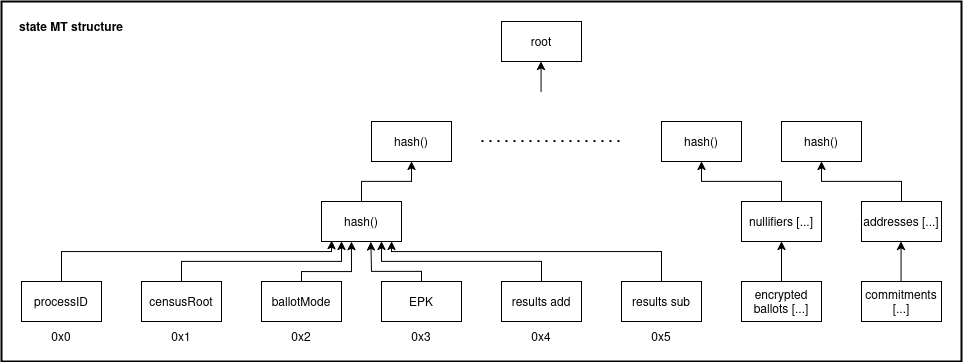
\includegraphics[width=400pt,draft=false]{\figs/mt-state}}
	\caption{Structure of the state Merkle tree (FIGURE SHOULD BE POLISHED).}
	\label{fig:mt-state}
\end{figure}

\textbf{The Initial State}: The voting process begins with an initial state where the Merkle Tree Root is established and published on the Process Management smart contract. Predefined parameters are included, but the results are initialized to zero, and no nullifiers are present. The Process Organizer transaction, contains the initial root and the necessary Merkle proofs. These proofs verify that the initial parameters are correct according to the voting process information and that no additional information is stored. Since the `ProcessId` of the initial state is a unique identifier, there won't be duplicate roots for different processes.


\subsubsection{Smart contracts}

\paragraph{Process management.} This smart contract is responsible for the life-cycle management of voting processes. It includes the initiation, monitoring, execution, and closure of voting events.

\paragraph{Sequencer registry.} For each voting process, this smart contract maintains the integrity of the cast votes and process life cycle. It verifies that each state transition committed by a sequencer adheres to the predefined rules.

\paragraph{Results verification.} This smart contract keeps track of the existing available sequencers, stores the collateral of the sequencers to ensure (that incentivizes) good behaviour, and is used to coordinate the distributed key generation when a new voting process is created.\\

\martai{This is wrong. Explanation of SR and RV smart contracts are mixed, I don't know what I was thinking when I wrote it. We should also include a sentence about the management of sequencers.}


\begin{figure}[h]
	\centerline{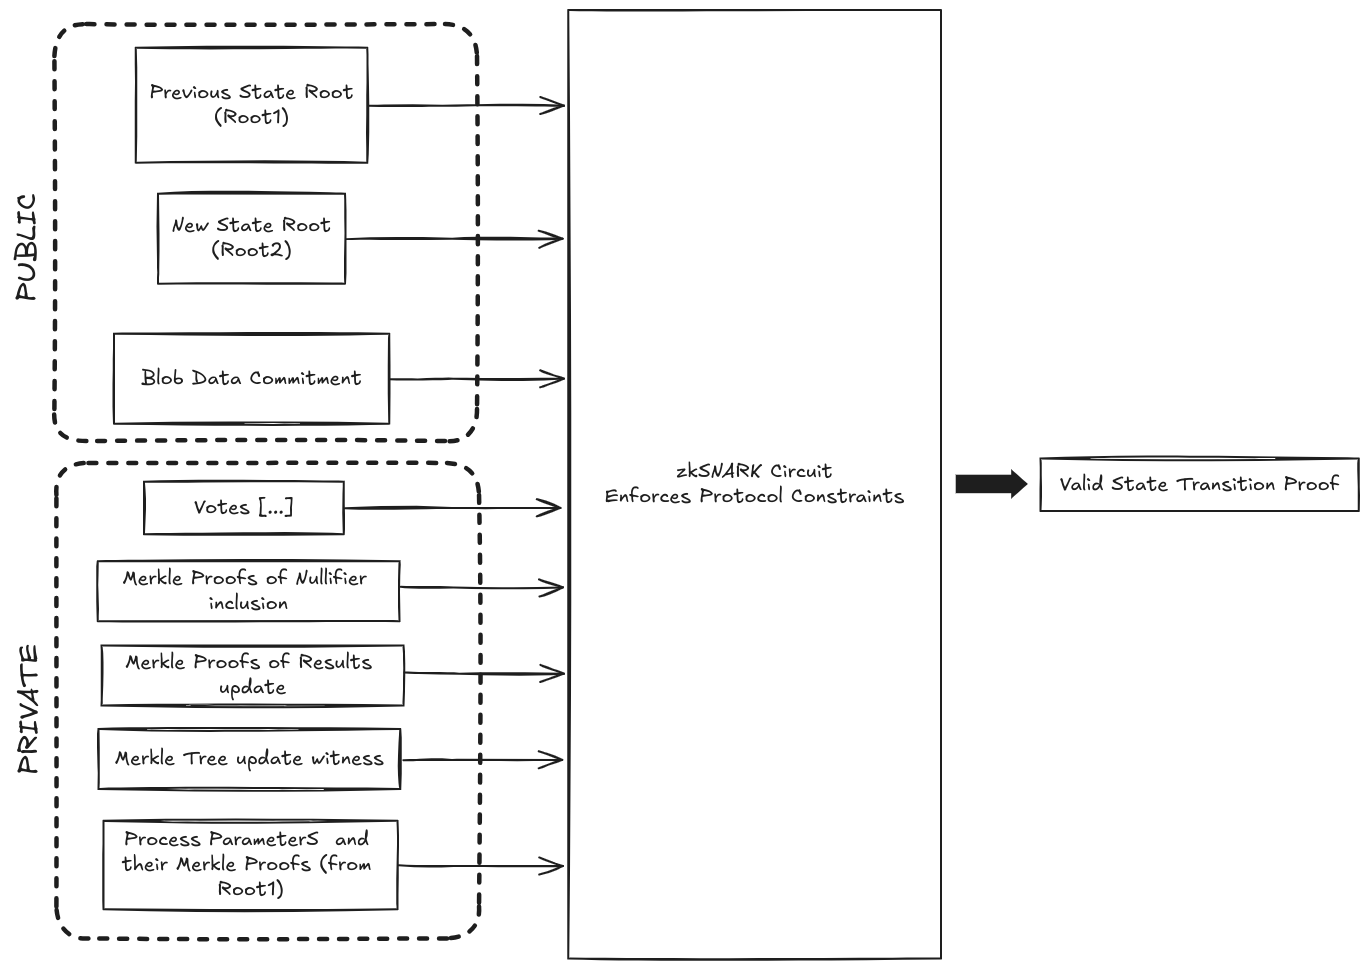
\includegraphics[width=400pt,draft=false]{\figs/circuit-inputs}}
	\caption{Caption.}
	\label{fig:circuit-inputs}
\end{figure}


\subsubsection{Votes [I don't think this is the right place]}

In the \davinci system, a vote comprises several components that work together to ensure secure, private, and verifiable voting. These components are:

\begin{enumerate}
	\item Process Identifier
	\item Census Proof
	\item Identity Commitment
	\item Nullifier
	\item Encrypted Ballot and Zero-Knowledge Proof (ZKP)
	\item Signature	
\end{enumerate}

Below, we detail each component and its role in the voting process.

\begin{enumerate}
	\item \textbf{Process Identifier} \\
	
	The \textbf{Process Identifier} (\texttt{ProcessId}) is a unique 32-byte number that uniquely identifies a specific voting process within the \davinci ecosystem. It encapsulates essential information, including the rules and constraints for ballots and the unique identifier of the \davinci blockchain instance.\\
	
	\item \textbf{Census Proof} \\
	
	The \textbf{Census Proof} serves as the voter's identity verification mechanism, ensuring that only eligible voters can participate. Depending on the process configuration, the voter provides:
	\begin{itemize}
		\item \textbf{Merkle Tree-Based Proof}: A Merkle proof showing inclusion in the census.
		\item \textbf{Credential Service Provider (CSP)}: A credential issued by a trusted third party. \\
	\end{itemize}
	
	\item \textbf{Identity Commitment}\\
	
	The \textbf{Commitment} $C$ is used to prevent a voter from registering multiple nullifiers and to avoid collisions if different voters choose the same secret.
	
	$$ C = \text{Hash} (\text{Address} || ProcessId || s). $$
	
	\begin{itemize}
		\item \textbf{Stored in State Merkle Tree (SMT)}: Indexed by the voter's address.
		\item \textbf{Prevents Multiple Registrations}: Each address can have only one commitment, ensuring a voter cannot register multiple secrets.
		\item \textbf{Collision Resistance}: Including the address in $C$ ensures that commitments are unique even if voters choose the same secret $s$.
	\end{itemize}
	
	The secret $s$ can be implemented from different ways or a combination of them, such as:
	
	\begin{itemize}
		\item A secure enough Password introduced by the user.
		\item A signature of a specific text.
		\item A random input that the user must store to allow potential vote overwrite.\\
	\end{itemize}
	
	\item \textbf{Nullifier} \\
	
	The \textbf{Nullifier} $N$ is a 32-byte hash used to:
	
	\begin{itemize}
		\item \textbf{Prevent double voting}: Ensures each voter can cast only one vote or overwrite their previous vote.
		\item \textbf{Allow vote overwrite}: Voters can submit a new vote with the same nullifier to replace their previous vote.
		\item \textbf{Provide anonymity}: Cannot be linked back to the voter's identity without knowledge of the secret $s$.
	\end{itemize}
	
	$$ N = \text{Hash}(\text{C} || s) $$ 
	
	\item \textbf{Encrypted Ballot and Zero-Knowledge Proof (ZKP)} \\
	
	The ballot contains the voter's selections encoded according to the ballot protocol rules. To ensure privacy, the ballot is encrypted using the ElGamal cryptosystem over elliptic curves, which allows homomorphic combination of encrypted votes.
	
	\textbf{Encryption process}:
	
	\begin{itemize}
		\item The voter's choice $m$ is encoded as a point on the elliptic curve.
		\item The voter selects a random scalar $k \in [1, n-1]$, where is the order of the elliptic curve group.
		\item Compute the ciphertext components:
		\begin{itemize}
			\item $C_1 = k \cdot G$
			\item $C_2 = M + k \cdot H$
		\end{itemize}
		\item The ciphertext is the pair $(C_1, C_2)$.
	\end{itemize}
	
	
	\textbf{Zero-Knowledge Proof (ZKP)}:
	
	The voter generates a ZKP to prove the correctness of the ballot and encryption process:
	
	\begin{enumerate}
		\item \textbf{Correctness of Encryption}: Ensures the ciphertext $(C_1, C_2)$ is correctly computed from the plaintext message $M$ and random scalar $k$.
		\item \textbf{Compliance with Ballot Protocol Rules}: The plaintext vote adheres to the ballot protocol constraints, such as valid choices and allowed number of selections.
		\item \textbf{Correct Computation of Commitment and Nullifier}:
		\begin{itemize}
			\item \textbf{Commitment}: $C = \text{Hash} (\text{Address} || ProcessId || s).$
			\item \textbf{Nullifier}: $N = \text{Hash}(\text{C} || s)$.
			\item The voter knows the secret linking the commitment and nullifier.
		\end{itemize}
	\end{enumerate}
	
	\textbf{Inputs to the ZKP Circuit}:
	
	\begin{itemize}
		\item \textbf{Public Inputs}:
		\begin{itemize}
			\item Encrypted Ballot $(C_1, C_2)$.
			\item Ballot Protocol Configuration.
			\item Encryption Parameters.
			\item Voter's Weight
			\item Commitment $C$.
			\item Nullifier $N$.
		\end{itemize}
		\item \textbf{Private Inputs}:
		\begin{itemize}
			\item Plaintext Vote $m$.
			\item Secret $s$.
			\item Random Scalar $k$.
			\item Voter's Address (used internally in the computation of $C$).
		\end{itemize}
	\end{itemize}
	
	\begin{figure}[H]
		\centering
		\fbox{
			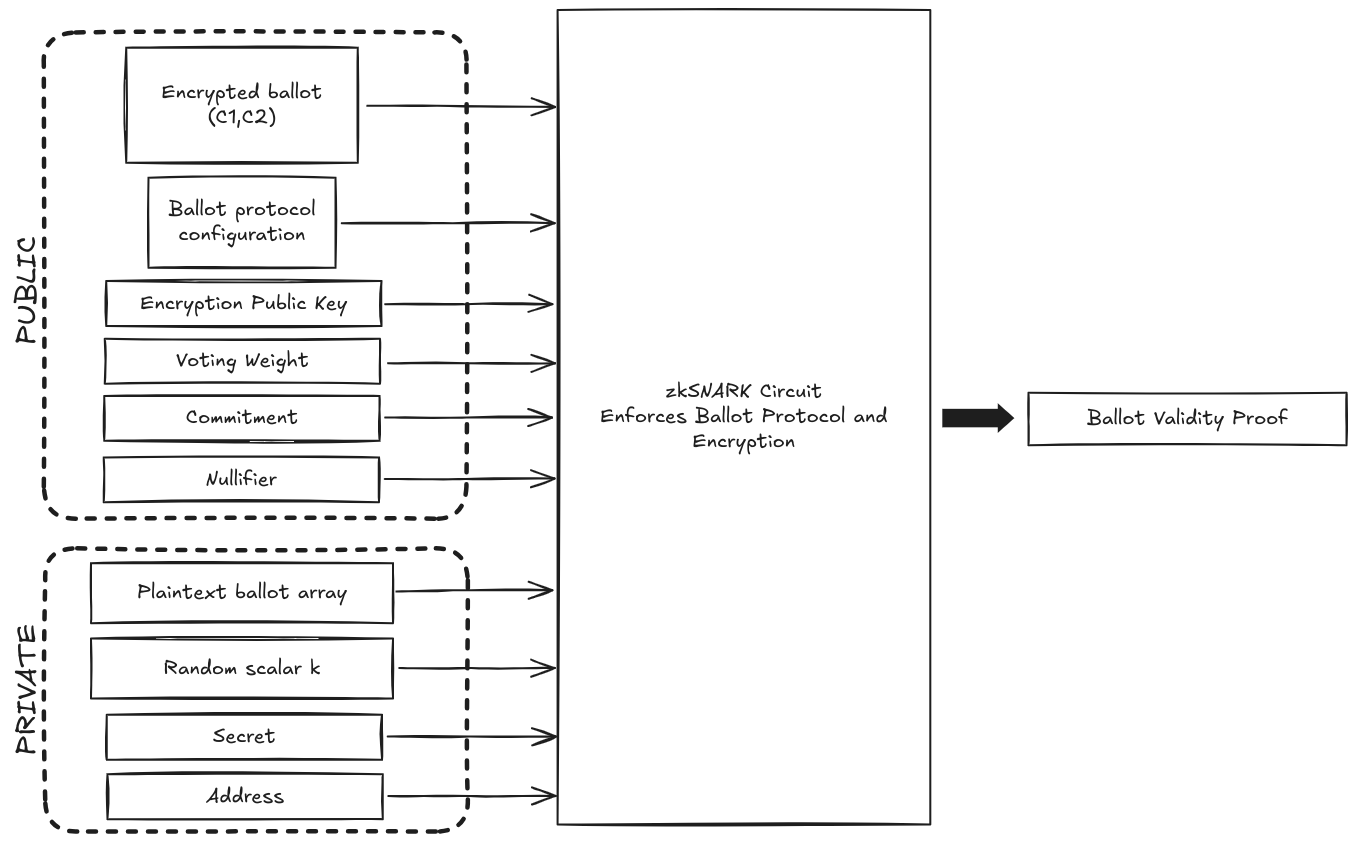
\includegraphics[scale = 0.3, draft = false]{\figs/vote-circuit-inputs.png}}
	\end{figure}
	
	\item \textbf{Signature}\\
	
	The \textbf{Signature} authenticates the vote and ensures that it was cast by a legitimate voter. The voter signs necessary components using their private key, depending on the census configuration (e.g., ECDSA, EdDSA, RSA).	
\end{enumerate}


\subsection{Circuits}
\label{sec:vocdoni-protocol:circuits}

\martai{The idea of this section is to describe de circuits. Then, in Section~\ref{sec:analysis:implementation} we give the details such as of the number of constants, framework used, etc. I haven't done this split yet.}

\textit{Old text: By structuring the process this way, we ensure that voting can be performed from any device-including smartphones and web browsers-while keeping the sequencer's computational requirements within the capabilities of accessible, CPU-based machines with 64 GiB of memory.}

\martai{I don't follow the above paragraph.}


\martai{NOTATION (1) What I name \texttt{config}, is called \texttt{Ballot Mode}, and (2) \texttt{MT root} is \texttt{census root}.}

\martai{It's convenient to name the proof associated to each circuit: a proof for this circuit is called [...] .}

\subsubsection{Voter circuit}

Figure~\ref{fig:circuit-voter}.

\paragraph{Description.} Generated by the user when casting a vote, this circuit proves that the encrypted ballot is valid (i.e. follows the protocol rules) and that the nullifier and commitment are correctly generated.

\begin{itemize}
	\item Constraints: Approximately 53.000
	\item Curve: BN254
	\item Framework: Circom/SnarkJS
	\item Actor: User
\end{itemize}

\paragraph{Assertions.}

\begin{itemize}
	\item \emph{Rules compliance}: The ballots meets the ballot mode provided following the protocol rules.
	\item \emph{Vote encryption}: The ballots encryption is correct.
	\item \emph{Vote commitment + nullification}: The nullifier and commitments are correctly computed.
\end{itemize}

\begin{figure}[h]
	\centerline{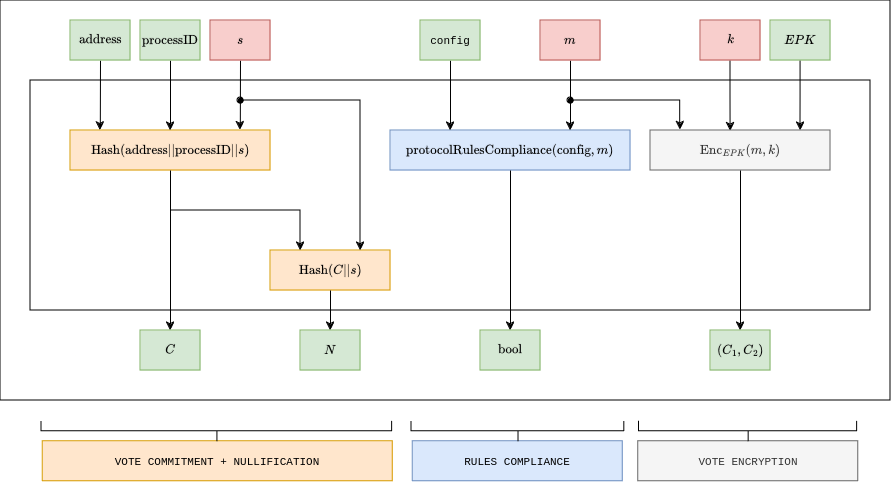
\includegraphics[width=400pt,draft=false]{\figs/voter-circuit}}
	\caption{Voter circuit. All public values are framed in green.}
	\label{fig:circuit-voter}
\end{figure}

\subsubsection{Authentication circuit}

Figure~\ref{fig:circuit-authentication}.

\paragraph{Description.} Generated by the sequencer, this circuit transforms the vote proof to the BLS12-377 curve for native recursion and validates the user's eligibility in the census, as well as their signature.

\begin{itemize}
	\item Constraints: Approximately 3.1 million
	\item Curve: BLS12-377
	\item Framework: Gnark
	\item Actor: Sequencer
\end{itemize}

\paragraph{Assertions.}

\begin{itemize}
	\item \emph{Voter's proof verification}: The vote zkProof is valid for the inputs provided.
	\item \emph{Authentication + non-malleability}: The signature of the inputs provided is valid for the public key of the voter.
	\item \emph{Census membership}: The address derived from the user public key is part of the census, and verifies the census proof with the user weight provided.
\end{itemize}

\begin{figure}[h]
	\centerline{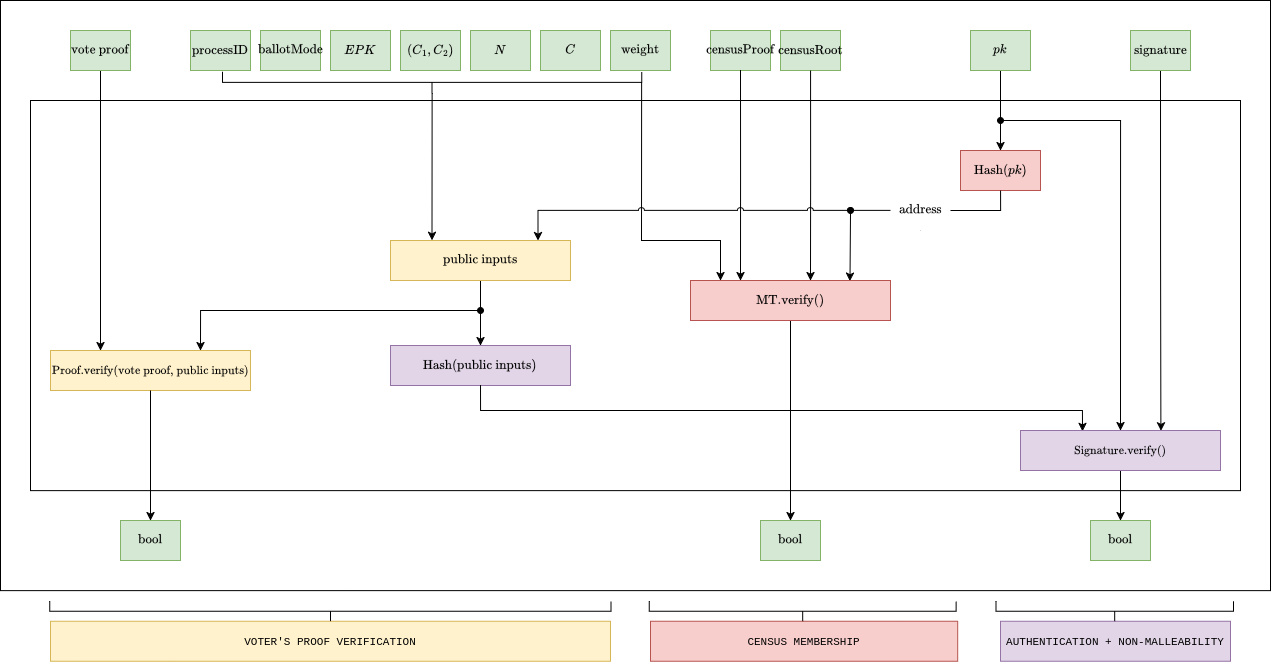
\includegraphics[width=400pt,draft=false]{\figs/circuit-authentication}}
	\caption{Authentication circuit. All public values are framed in green.}
	\label{fig:circuit-authentication}
\end{figure}

\subsubsection{Aggregation circuit}

Figure~\ref{fig:circuit-aggregate}.

\paragraph{Description.} This circuit accumulates multiple authenticated votes into a single proof. It also verifies that all accumulated votes belong to the same voting process.

\begin{itemize}
	\item Constraints: 40.000 $\times$ (number of votes)
	\item Curve: BW6-761
	\item Framework: Gnark
	\item Actor: Sequencer
\end{itemize}

\paragraph{Assertions.}

\begin{itemize}
	\item \emph{Votes aggregation}: The accumulated zkProofs are valid.
	\item \emph{Shared public inputs}: The ProcessId, CensusRoot, BallotMode and EPK is the same for all of them.
\end{itemize}

\begin{figure}[h]
	\centerline{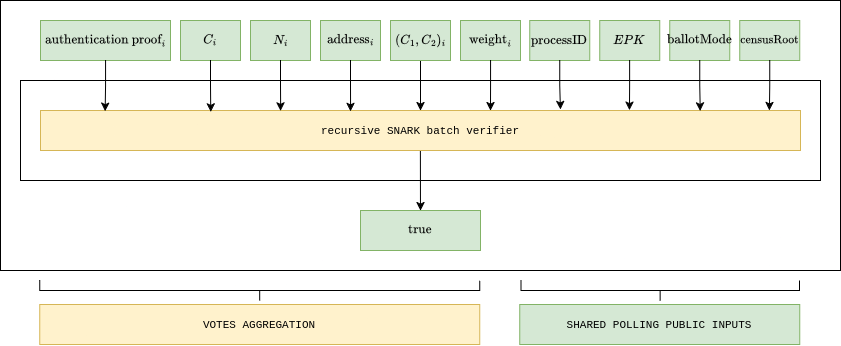
\includegraphics[width=400pt,draft=false]{\figs/circuit-aggregate}}
	\caption{Aggregation circuit. All public values are framed in green.}
	\label{fig:circuit-aggregate}
\end{figure}


\subsubsection{State transition circuit}

\paragraph{Description.} Given the aggregated votes proof, this circuit verifies the correct inclusion of all new votes into the process's state Merkle tree. It generates the final state transition proof that will be validated by the Ethereum smart contract.

\begin{itemize}
	\item Constraints: Approximately 4 million
	\item Curve: BN254
	\item Framework: Gnark
	\item Actor: Sequencer
\end{itemize}

\paragraph{Assertions.}

\begin{itemize}
	\item \emph{Aggregation verification}: The agreggated zkProof is valid.
	\item \emph{Transition verification}: The MerkleTree transition witness proves every change between Root1 and Root2.
	\item \emph{Public inputs integrity}: ProcessID, BallotMode, CensusRoot, EncryptionKey remain unchanged.
	\item \emph{Votes counting}: Ballots are correctly counted as new or overwrites, and added to results accumulators.
\end{itemize}

\martai{The corresponding circuit figure is not done yet.}

\noi \textit{Old original text, I think it will help here:}

When a new voting process begins, the Sequencer initializes a new State, represented by the root hash of a Merkle tree. This tree encapsulates all essential information about the voting process, including process parameters, voter registry (census), ballot configurations, and initial results.

For each new batch of votes, the Sequencer updates the state by generating a zkSNARK proof that \textbf{validates the state transition from the current Root to a new Root}. This proof is submitted on-chain for settlement. By doing so, we maintain an immutable and verifiable record of the voting process on the blockchain.

This approach allows anyone to access the latest verified state of the voting process from the Results Verification smart contract, along with the necessary data to process subsequent state updates. The system's design enables multiple Sequencers to participate in tallying votes. They can take the current State Root and its associated data to construct the next state, incorporating new votes into the tally. This decentralization of Sequencers helps prevent potential censorship and reinforces the robustness of the voting process.

\paragraph{Maintaining the Chain.}

The chain of integrity is maintained through a combination of smart contract enforcement and strict zkSNARK circuit constraints. This ensures that each state transition is valid and builds upon the last accepted state without requiring additional mechanisms.

\begin{itemize}
	\item \textbf{Sequential State Roots}: Each state transition updates the Merkle tree from a previous root (`Root1`) to a new root (`Root2`) after processing a batch of votes.
	\item \textbf{Smart Contract Enforcement}: The smart contract verifies that the `Root1` provided in the zkSNARK proof matches the last committed state root stored on-chain. This guarantees that all transitions are sequential and based on the latest accepted state.
	\item \textbf{Proof Validation}: The smart contract uses the zkSNARK verification key to validate the submitted proof. A valid proof confirms that the transition from `Root1` to `Root2` adheres to all protocol rules enforced by the circuit.
	\item \textbf{State Update}: Upon successful verification, the smart contract updates the stored state root hash to`Root2`, ensuring an immutable and continuous chain of states.
\end{itemize}

\paragraph{State Transition}

To validate and process state transitions, \textbf{we employ a zkSNARK circuit that enforces all protocol constraints}. This circuit proves that the transition from the previous state Root to the new state Root is valid based on the newly processed votes.

\begin{figure}[H]
	\centering
	\fbox{
		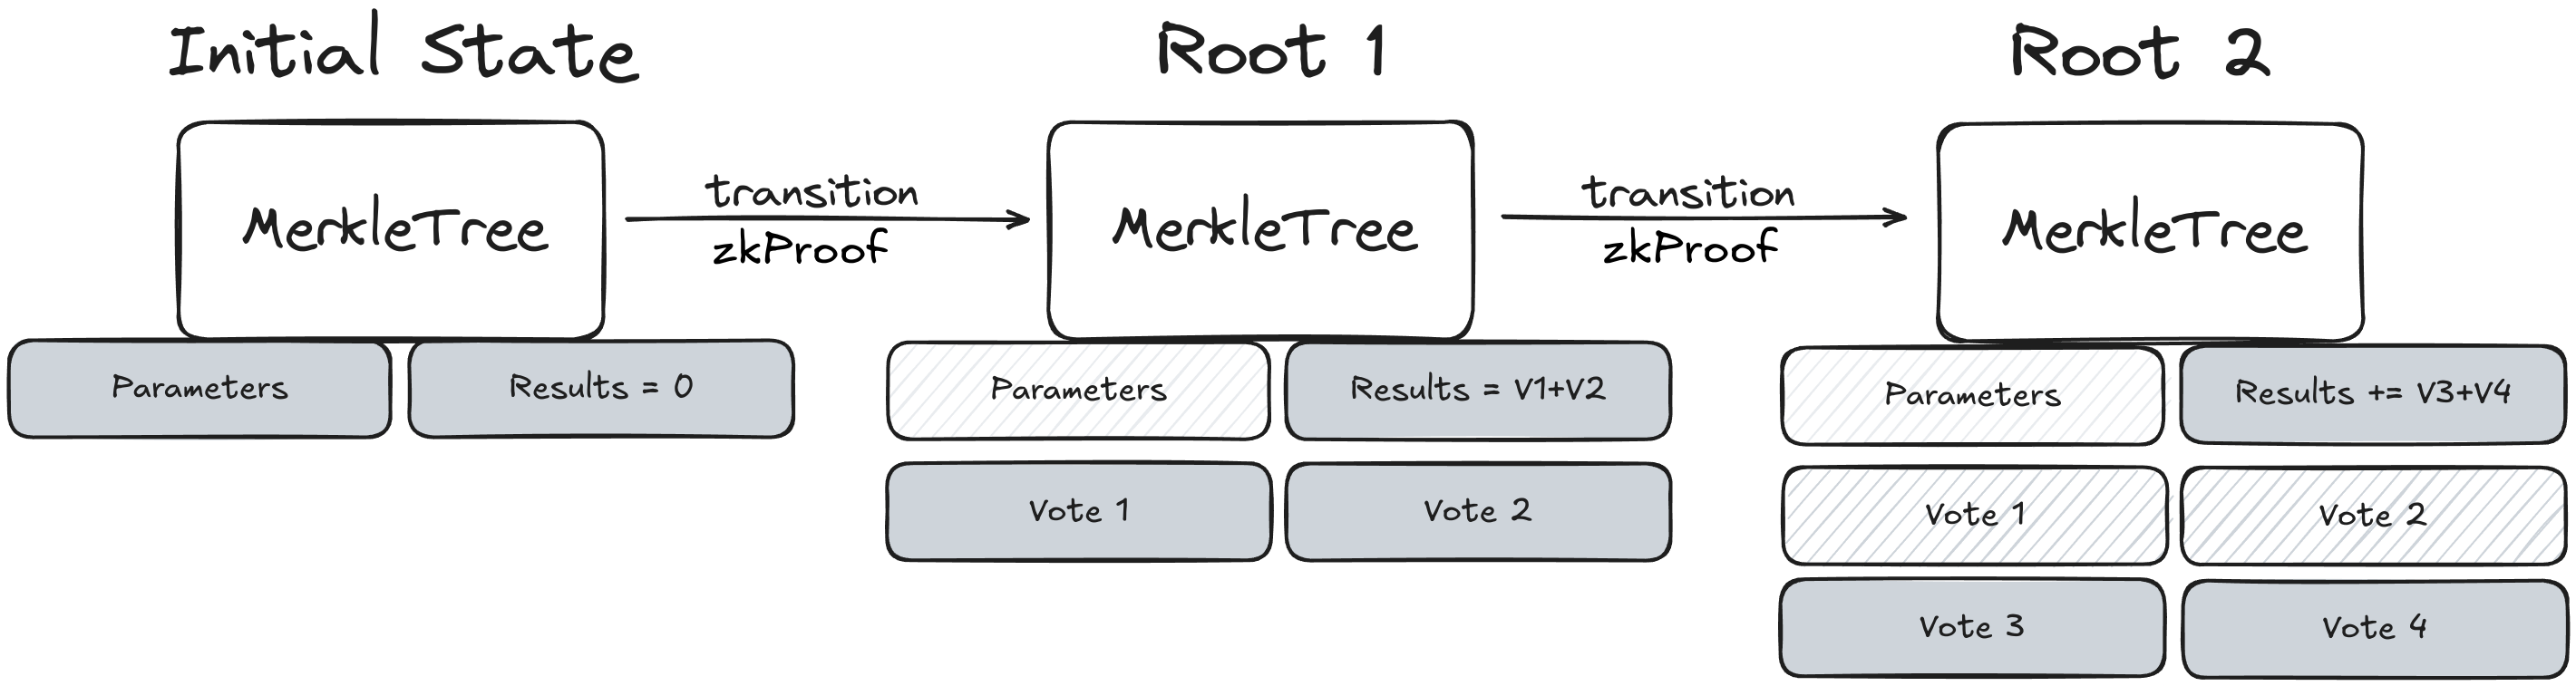
\includegraphics[scale = 0.12, draft = false]{\figs/state-transition.png}}
\end{figure}

The circuit have the following inputs (the public ones are required to verify the proof).

\begin{itemize}
	\item \textbf{Public Inputs:}
	\begin{itemize}
		\item Previous State Root (Root1): The Merkle tree root before the state transition.
		\item New State Root (Root2): The Merkle tree root after the state transition.
		\item Blob Data Commitment (blobCommitment): The commitment to the data blob containing the new votes.
	\end{itemize}
	\item \textbf{Private Inputs:}	
	\begin{itemize}
		\item Votes: The list of new votes being processed, including census proofs and authentication data.
		\item Merkle Proofs of nullifier inclusion: Proofs that each voter nullifier is included in the census.
		\item Merkle Proofs of results update: Proofs that the process results have been correctly updated.
		\item Merkle Tree Update Witnesses: Necessary data (e.g., Merkle paths) to update the Merkle tree from Root1 to Root2.
		\item Process Parameters: Retrieved from Root1 within the circuit.
	\end{itemize}
\end{itemize}

\begin{figure}[H]
	\centering
	\fbox{
		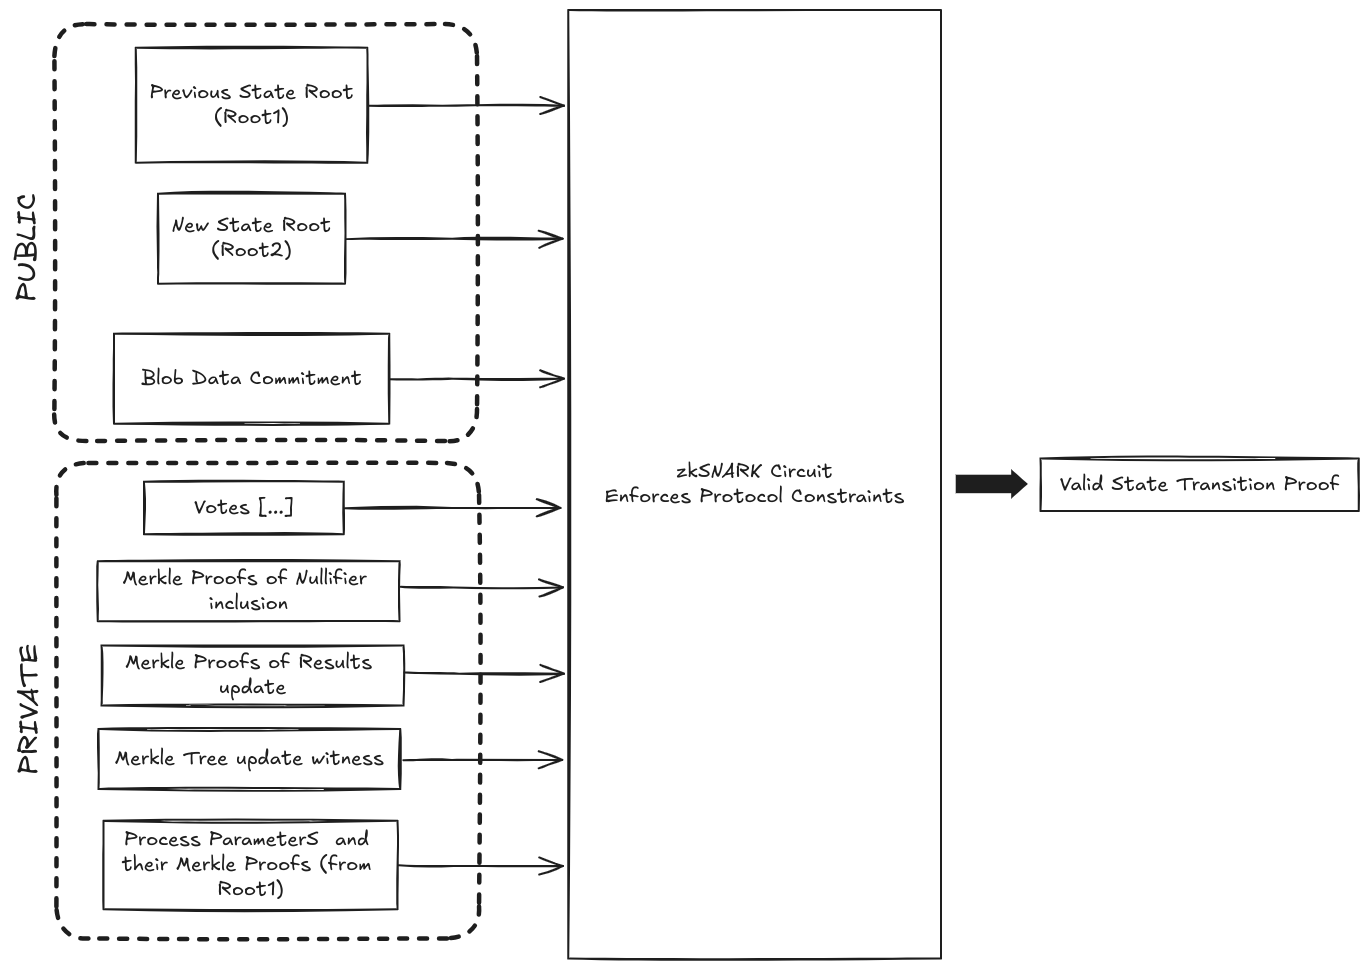
\includegraphics[scale = 0.3, draft = false]{\figs/circuit-inputs.png}}
\end{figure}

The following constraints must be enforced by the circuit.

\begin{itemize}
	\item \textbf{Immutable Process Parameters}: Ensure that critical process parameters (such as `censusRoot` or `processId`) retrieved from `Root1` remain consistent and are not altered in the transition.
	\item \textbf{Vote Validity}: Validate that each vote proof is correct.
	\item \textbf{Voter Eligibility}: Confirm that each voter is included in the census by verifying Merkle proofs of inclusion against the `censusRoot` retrieved from `Root1`.
	\item \textbf{Nullifier Non-Existence}: Ensure that the nullifier for each vote does not exist in the current state (`Root1`), preventing double voting.
	\item \textbf{Nullifier Addition}: Correctly add each new nullifier to the state, resulting in `Root2`, updating the Merkle tree accordingly.
	\item \textbf{Results Update}: Ensure that the voting results are accurately updated by adding the new votes to the previous results retrieved from `Root1`, so that `results2 = results1 + votes`.
	\item \textbf{Blob Data Integrity}: Confirm that the data used in the circuit (votes, nullifiers) corresponds to the `blobCommitment` provided as a public input, ensuring that the votes processed are exactly those published in the data blob.
	\item \textbf{State Transition Validity}: Ensure that the new state root (`Root2`) is correctly computed from `Root1` by applying the validated votes and updates to the Merkle tree.
\end{itemize}

\subsection{Protocol flow}
\label{sec:vocdoni-protocol:flow}

In Figure~\ref{fig:protocol-flow} we describe the protocol flow.

\martai{About the figure: layout should be fixed. In addition, the icons for the different parties are missing.}

\begin{figure}[H]
	\centerline{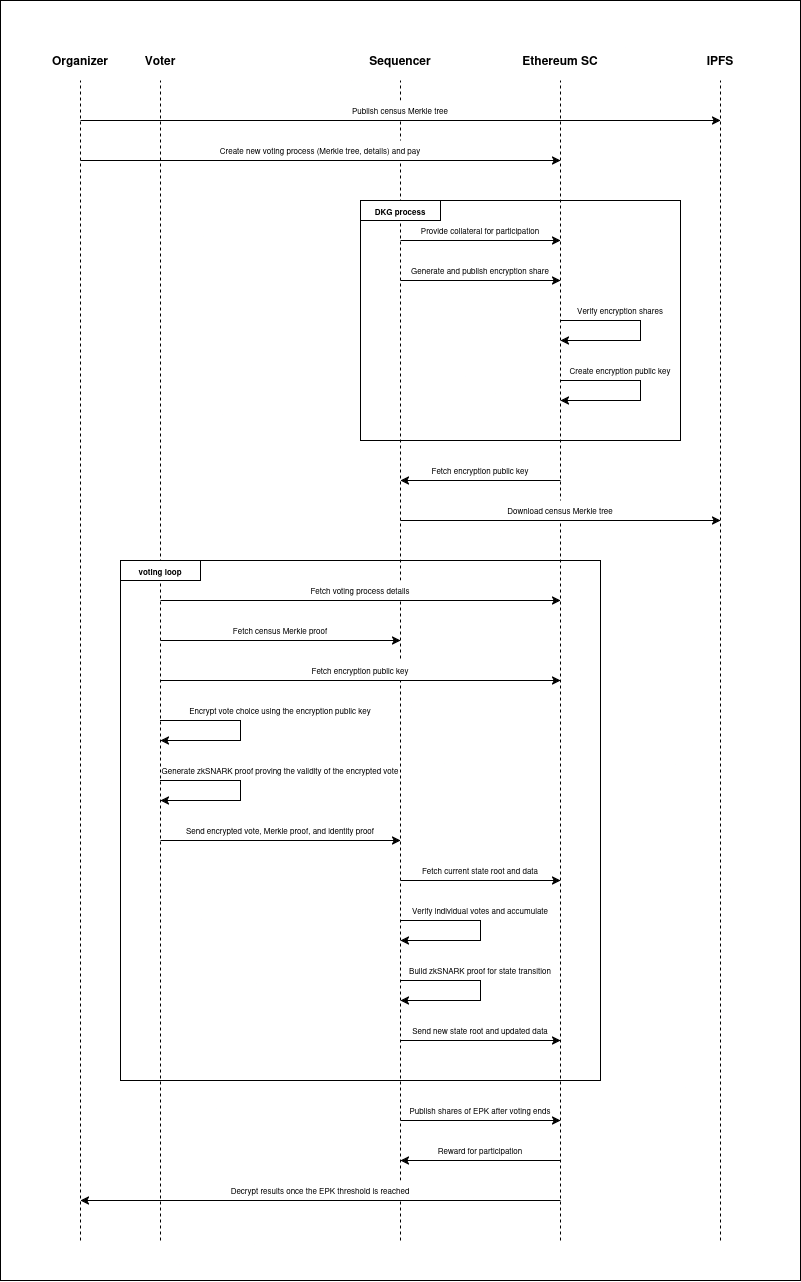
\includegraphics[width=400pt,draft=false]{\figs/protocol-flow}}
	\caption{Vocdoni voting process overview.}
	\label{fig:protocol-flow}
\end{figure}

\subsection{Prior to voting (only once)}
\label{sec:vocdoni-protocol:prior-steps}

\martai{Remove the first step, we assume contracts are already deployed or at least, the logic is available.}

This is done only once. Then every voting will start its process from step in Section~\ref{sec:vocdoni-protocol:start}.

Vocdoni:
\begin{enumerate}
	\item Deployment of the 3 smart contracts.
	\item Sequencers registry starts (it doesn't end).
\end{enumerate}

Sequencers (nodes validadors) -- this process is always open:
\begin{enumerate}
	\item Register this and that way.
	\item Public keys?
	\martai{Sequencers must also publish how they can be reached (either when they register or when they contribute to the DKG). They can use a URI: Uniform Resource Identifier.}
	\item PROVIDE COLLATERAL.
	\martai{What happens to the collateral? If done only once, then you lose it? Do you need to send a new tx with more collateral?}
	\item Send transaction to Sequencer registry smart contract (pay for tx fee).
\end{enumerate}

\subsection{Start of the voting process}
\label{sec:vocdoni-protocol:start}

The organizer:
\begin{enumerate}
	\item Prepares the census data \texttt{census\_data}.
	\item Generates the census commitment \texttt{MT\_census.root = Com(census\_data)}.
	\martai{In general, make use (link) to the functions defined in Section~\ref{sec:cryptographic-primitives}. For example, here the \texttt{MT.root()}.}
	\martai{Additionally, after this step, the organizer should make a Merkle proof available to all eligible voters.}
	\item Set voting details: duration, options, type, etc. + CENSUS MT ROOT.
	\item Also a timeout for the DKG ceremony + minimum number of sequencers.
	\item Send transaction to the Ethereum process management smart contract with all data. Note this transaction has a cost (Eth tx fees) that needs to be covered by the organizer.
\end{enumerate}

\subsection{Key generation process} %Voting key generation
\label{sec:vocdoni-protocol:dkg}

The sequencer:
\begin{enumerate}
	\item Download all required data from the PM smart contract which includes the census MT root to handle the new vote.
	\item Make contributions to DKG ceremony.
\end{enumerate}

After XXX time (set by the organizer in the PM contract?): all contributions to DKG are done.

\martai{The organizer decides a minimum number of sequencers (security factor).}
	
\begin{itemize}
	\item EPK ``becomes available".
	\martai{I understand EPK becomes available in the SR smart contract, and that key is sent to the PM contract?}
	\martai{The idea here is that some sequencer makes EPK available (a.k.a. sends a transaction). Alternatively, generate a SNARK proving the EPK has been generated correctly and the SC verifies it.}
\end{itemize}

\subsection{Voting process}
\label{sec:vocdoni-protocol:voting}

Voter:

\begin{itemize}
	\item Choose any of the available sequencers (from?? -- from the SR SC).
	\item Fetch their census \textbf{Merkle proof} to prove eligibility (from the census registry).
	\item Use the EPK to encrypt the voting choice.
	\item Generate ZK-SNARK of satisfiability of circuit from Fig.~\ref{fig:circuit-voter} with protocol from Section~\ref{sec:cryptographic-primitives:zkp} to prove the validity of the encrypted vote and adherence to ballot protocol rules. We call this proof \textbf{vote proof}.
	\item Send the encrypted vote, Merkle proof, validity proof, and identity proof to the sequencer.
	\martai{I understand Validity proof refers to ``voter circuit"? Merkle proof is for inclusion, right? And identity proof is for example a signature??}
\end{itemize}

Sequencer:

\begin{itemize}
	\item Fetch current state: retrieve the current valid process state root from the Etherem smart contract and the associated data from Ethereum blobs.
	\martai{specify which SC.}
	\item Generate a SK-SNARK proof of state transition proving:
		\begin{itemize}
			\item the validity of the ZK-SNARK proof provided by the voter,
			\item the correct accumulation of votes from users, adding them to the process state,
			\item the correct sum of the new encrypted votes using the homomorphic properties of ElGamal,
			\item the new votes are from eligible users by checking the census Merkle proofs,
			\item the new voters have not already voted by checking their nullifiers, or it is a correct vote overwrite,
			\item the data blob hash matches the data used to verify the transition.
		\end{itemize}
	\item Submit updated state: send the new state root to the smart contract and store the updated data in Ethereum blobs.
\end{itemize}

Sequencers keep accumulating votes and create state transition until the finalization of the process.

\martai{I understand this finalization is a deadline set by the organizer.}

SC:

\begin{itemize}
	\item Upon receiving a sequencer's transaction, the SC verifies the zk-SNARK proof provided byt he sequencer.
	\item Ensure the origin root corresponds to the current stored state root.
	\item Confirm that the blob hash matches the one stored in Ethereum.
\end{itemize}

\subsection{Results validation}
\label{sec:vocdoni-protocol:validation}

Once the voting is completed (I understand the timeout set by the organizer expires), the following things happen.

Sequencer:

\begin{itemize}
	\item $t$ out of $n$ sequencers publish their shares corresponding to the EPK to the Ethereum smart contract.
	\martai{specify which SC.}
	\item When the threshold of shares is reached, the results can be decrypted by anyone.
	\martai{mention that the SC computes the corresponding ESK, or that can be computed by anyone off-chain, since all info is public.}
	\item Sequencers receive reward for their correct participants depending on the number of sequenced votes.
	\martai{slash if they don't provide the right share? reward only dependent of sequenced votes? any relation to their participation in the computation of either EPK or ESK?}
\end{itemize}

This way:

\begin{itemize}
	\item After the voting period ends and the results are decrypted, anyone can verify the correctness of the final result.
	\martai{explain how.}
	\item Use the zkSNARK state proof and publicly available data on-chain to ensure the integrity and correctness of the entire voting process.
	\martai{elaborate on this.}
\end{itemize}

\subsection{Finalization of the voting process}
\label{sec:vocdoni-protocol:finalization}


\section{Ballot protocol}
\label{sec:ballot-protocol}
% !TeX root = ../build/main.tex

\martai{All this section is the original old text.}

The \textit{Vocdoni ballot protocol} is a simple and efficient mechanism for casting and tallying votes in any type of election or collective decision-making process. Each voting process consists of one or several fields and voters are required to provide a response for each of these fields in their ballot.

The responses in the ballot are represented as a sequence of natural numbers, each corresponding to the voter’s choice for the respective field. Results are accumulated into a single array. Each position in the array corresponds to the sum of all votes cast for that field across all voters.

The ballot protocol is defined by a set of configurable variables that dictate how votes must be cast. This way the protocol can accommodate a wide range of voting processes and behaviors.

\begin{enumerate}
	\item \maxcount: Defines the maximum number of fields in a ballot (max 64).
	\item \maxvalue: The maximum allowable value for any field in a ballot (if greater than 0).
	\item \minvalue: The minimum allowable value for any field in a ballot (default 0).
	\item \uniquevalues: Specifies whether voters can select the same value multiple times within a ballot (default false).
	\item \maxtotalcost: Limits the sum of all field values in a ballot (if greater than 0).
	\item \mintotalcost: Specifies a minimum required total sum of field values in a ballot (default 0)
	\item \costexponent: Defines the exponent used to calculate the "cost" of votes for each field (default 1
\end{enumerate}

\begin{figure}[H]
	\centering
	\fbox{
		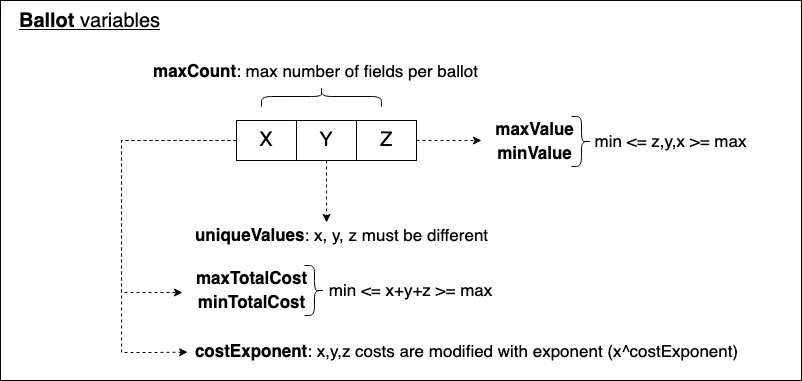
\includegraphics[scale = 0.4, draft = false]{\figs/ballot-variables.png}}
\end{figure}

\paragraph{Example 1: Rating candidates.}

Consider a voting process where voters are asked to rate three candidates: Lennon, Hendrix, and Joplin. Voters rate each candidate from 0 to 5 stars, and each vote is represented as an array where each position corresponds to the candidate’s rating. The configuration of this voting would be the following:

\begin{itemize}
	\item \maxcount: 3
	\item \maxvalue: 5
	\item \uniquevalues: Yes
\end{itemize}

Ballots:

\begin{itemize}
	\item Vote 1: \texttt{[3, 2, 5]} (3 stars for Lennon, 2 stars for Hendrix, 5 stars for Joplin)
	\item Vote 2: \texttt{[4, 3, 2]}
	\item Vote 3: \texttt{[2, 4, 5]}
\end{itemize}

After accumulating the votes:

\begin{itemize}
	\item Results Array: \texttt{[3+4+2, 2+3+4, 5+2+5] = [9, 9, 12]}\\
	Lennon received 9 points, Hendrix received 9 points, and Joplin received 12 points.
\end{itemize}

\paragraph{Example 2: Quadratic voting for resource allocation.} 

In a scenario where voters distribute a fixed number of credits across different options (e.g., selecting funding levels for NGOs), the ballot allows voters to assign multiple points, but the cost of casting multiple votes for a single option increases quadratically.

Configuration:

\begin{itemize}
	\item \maxcount: 4
	\item \maxtotalcost: 12 (credits)
	\item \costexponent: 2 (quadratic)
\end{itemize}

Ballots:

\begin{itemize}
	\item Vote 1: \texttt{[2, 2, 2, 0]}
	\item Vote 2: \texttt{[1, 1, 3, 1]}
	\item Vote 3: \texttt{[0, 2, 1, 2]}
\end{itemize}


After accumulating the votes:


\begin{itemize}
	\item Results Array: \texttt{[2+1+0, 2+1+2, 2+3+1, 0+1+2] = [3, 5, 6, 3]} \\
	Each position in the array represents the total sum of credits allocated to each NGO.
\end{itemize}

\martai{Cost may be dependant on the voter's weight.}

\section{The Vocdoni token}
\label{sec:token}
% !TeX root = ../build/main.tex

\Davinci introduces the Vocdoni token (\token) as a key element of its decentralized voting ecosystem, playing a crucial role in the protocol's sustainability.
The token serves multiple utility functions that align the incentives of all participants (voting organizers, sequencers, and voters) ensuring the integrity, efficiency, and security of the voting system.

\subsection{Roles of the \token}

\begin{enumerate}
	\item \textbf{Collateral for sequencers}: Sequencers are required to stake \token tokens as a collateral to participate in the protocol. This serves as a safeguard to ensure responsible participation. If a sequencer behaves improperly (whether due to malicious intent or unintentional errors) it can face penalties, including the loss of part of its staked tokens.
	\item \textbf{Incentive mechanism}: Sequencers earn rewards in \token tokens based on their contribution to processing valid votes and maintaining the network. Rewards are proportional to the number of valid votes successfully added to the shared state.
	\item \textbf{Payment for voting processes}: Voting processes organizers use \token tokens to cover the costs of creating and managing voting processes. The costs depend on factors like the size of the voting registry, the voting period's duration, and the desired level of security (based on the number of participating sequencers).
	\item \textbf{Governance}: The \token token facilitates decentralized governance by giving the token holders the right to participate in the project governance. Token holders can influence on important matters such as protocol upgrades, ecosystem development, and other initiatives aimed to enhance various aspects of \davinci. This ensures that the project evolves in a transparent, community-driven manner.
\end{enumerate}

\subsection{Economics for organizers}

Organizers of voting processes pay fees in \token tokens to create and manage their voting events. These fees cover operational costs and incentivize the sequencers.

The costs of voting processes vary based on the following factors:

\begin{itemize}
	\item \textbf{Maximum number of votes}: Larger voter registries require more resources for processing.
	\item \textbf{Voting duration}: Longer voting periods demand extended resource commitments from sequencers.
	\item \textbf{Security level}: Organizers can adjust the number of participating sequencers to balance between cost and security needs.
\end{itemize}

Fees must be paid upfront but can be partially reimbursed. The formula for calculating the reimbursement is:

$$ \reimbursement = \totalCost - \totalReward - \baseCost $$

Given that there is a list of eligible voters for each voting process, organizers should reserve space equal to the maximum number of voters, anticipating that all eligible voters may participate. However, since this is unlikely, a portion of the reward pool may be reimbursed.

The components of this formula are defined in the following sections.

\subsection{Voting process cost model}

The process cost model defines how the cost for a given process is calculated.
Considering sequencer-specific capacities, process duration, number of voters and security costs, we define following components formula:

$$ \totalCost = \baseCost + \capacityCost + \durationCost + \securityCost $$

\subsubsection{Components definition}

\begin{itemize}
	\item $\baseCost$: The base cost is a fixed fee charged by the sequencer to set up a voting process based on a fixed value plus the number of and a fixed factor. It is independent of the process duration, or the security level. This part cannot be reimbursed thus is a portion of the that will alwways be rewarded to the sequencers.
	$$ \baseCost = \fixedCost + \maxVotes \cdot p $$
	Where:
	\begin{itemize}
		\item $\fixedCost$ is a fixed base fee defined into the protocol.
		\item $\maxVotes$ is the maximum number of votes of a given voting process.
		\item $p$ is a small lineal factor defined into the protocol.
	\end{itemize}
	
	\item \capacityCost: It defines the cost given the current occupancy of the sequencer network. This component models the cost of reserving space for voting processes, relative to the number of sequencers available, the number of running voting processes and the maximum numbers of voters. The cost increases non-linearly as the number available sequencers approaches to the total number of sequencers and the number of running voting processes grows, so when there are fewer sequencers available and big number of voting processes running, the capacity becomes more valuable.
	$$
	k_1 \cdot \left( \frac{\totalVotingProcesses}{\totalSequencers - \usedSequencers + \epsilon} \cdot \maxVotes \right)^a
	$$ 
	\begin{itemize}
		\item $k_1$: A scaling factor controlling the impact of sequencers usage.
		\item $\totalVotingProcesses$: The total number of running voting processes.
		\item $\totalSequencers$: The total number of registered sequencers.
		\item $\usedSequencers$: The number of sequencers that are already handling other voting processes.
		\item $a$: An exponent that controls how sharply the cost increases as the used capacity approaches the total available capacity. In other words, it controls the non-linearity of the cost increase.
		\item $\epsilon$: Is a very small number that avoids zero division.
	\end{itemize}
	
	\item $\durationCost$: This component models the cost of running the process for a specific duration, where longer processes incur into more cost. The scaling is non-linear, meaning that shorter processes are more cost-efficient, while longer processes are increasingly expensive.
	
	It is expected to have a minimum and maximum duration thresholds (e.g 1 hour to 1 year).
	
	$$ k_2 \cdot \processDuration^b $$
	
	\begin{itemize}
		\item $k_2$: A scaling factor for the process duration.
		\item $\processDuration$: The duration of the process in hours.
		\item $b$: An exponent that controls the non-linear scaling of the process duration.
	\end{itemize}
	
	\item $\securityCost$: The security cost models the use of multiple sequencers to ensure a secure process. The cost scales exponentially based on the number of sequencers used, but with diminishing returns as the number of sequencers approaches the total available sequencers:
	
	$$ k_3 \cdot e^{c \cdot \left( \frac{\numSequencers}{\totalSequencers} \right)^d} $$
	
	\begin{itemize}
		\item $k_3$: A scaling factor controlling the overall weight of security cost.
		\item $c$: Controls the steepness of the exponential scaling for security costs.
		\item $\numSequencers$: The number of sequencers used in this process.
		\item $\totalSequencers$: The total number of available sequencers in the network.
		\item $d$: An exponent controlling how fast the security cost increases as the number of sequencers approaches the total available sequencers.
	\end{itemize}
\end{itemize}

\subsubsection{Constraints}

There is the need to enforce some constrains in the formula in order to avoid impracticable scenarios.

\begin{itemize}
	\item If $\processDuration > \maxDuration$ then: $\totalCost = \infty$.
	\item If $\numSequencers > \totalSequencers$ then: $\totalCost = \infty$.
\end{itemize}

\subsection{Economics for sequencers}

To become a sequencer and earn rewards, participants must stake \token tokens as collateral. This collateral is locked during the sequencer registry in the Sequencer Registry smart contract and can be withdrawn upon the sequencer commitments are fulfilled.

Sequencers \textbf{receive rewards} based on:

\begin{itemize}
	\item The number of \textbf{votes} they include in the shared state.
	\item The number of \textbf{vote rewrites} they include in the shared state.
	\begin{itemize}
		\item A vote rewrite can be either a vote overwrite (a voter casting another vote that overwrites the previous one) or a vote re-encryption (made by the sequencer). Rewriting votes enables more flexibility for the voter and is a key mechanism for the receipt-freeness.
		\item It is expected for the sequencers to maximize the number of vote rewrites because there is no way to distinguish between a vote overwrite and a vote re-encryption. This is considered a positive behavior because it contributes to the receipt-freeness mechanism of the protocol.
		\item A vote and a vote rewrite are distinguishable because the former include a nullifier that has not ever been included in a specific process.
		\item Given that each sequencer will submit a ZK proof validating the state transition into the settlement layer smart contract it is straight forward to count the number of votes and the number of vote rewrites processed by each sequencer.
		\item Sequencers can allow vote rewrites up to $T$ times the number of new votes for any state transition. $T$ will be defined as a constant in the protocol.
	\end{itemize}
	\item The number of \textbf{non-processed votes} in relation to the maximum number of voters.
\end{itemize}

The total reward obtained can be expressed as:

$$ \sequencerReward_i = R \cdot \left( \frac{\votes_i}{\maxVotes} \right) + W \cdot \left( \frac{\voteRewrites_i}{\totalRewrites}  \right) $$

And subject to the constraints:

$$ \frac{\voteRewrites_i}{\votes_i} \leq T$$

$$ \totalReward = R + W $$

$$ R > W $$

\begin{itemize}
	\item $R > W$ since the sequencers must prioritize processing votes and not be incetivized to just rewrite existing votes.
\end{itemize}

Where:

\begin{itemize}
	\item $R$: A part of the reward pool allocated for a specific voting process.
	\item $\votes_i$: The number of votes processed by the sequencer for a specific voting process.
	\item $\maxVotes$: The maximum number of voters participating in a voting process.
	\item $W$: A part of the reward pool allocated for a specific voting process.
	\item $\voteRewrites_i$: The number of vote rewrites processed by the sequencer for a specific voting process.
	\item $\totalRewrites$: The total number of vote rewrites for a specific process.
\end{itemize}

\subsubsection{Penalties}

\begin{itemize}
	\item Non-participation: Sequencers who fail to meet their obligation, not providing key shares during the tally phase, can have their collateral slashed.
	Penalites for a sequencer can be expressed as:
	$$ \slashedAmount_i = s \cdot \stakedCollateral_i $$
	Where:
	\begin{itemize}
		\item $\slashedAmount_i$: The total slashed amount for a given sequencer.
		\item $s$: The slashing coefficient $0 \leq s \leq 1$.
		\item $\stakedCollateral_i$: The amount of \token tokens staked by a given sequencer.
	\end{itemize}
\end{itemize}

\subsection{Summary}

The total cost formula combines four main components:

\begin{enumerate}
	\item A base cost for setting up the process.
	\item A capacity cost based on the number of voters, the total running processes and available sequencer capacity.
	\item A duration cost based on how long the process lasts.
	\item A security cost based on the number of sequencers used, with diminishing returns for using more than a certain number.
\end{enumerate}

The proposed formula ensures that:

\begin{itemize}
	\item Small processes are cost-efficient.
	\item Larger processes or processes using a high proportion of available sequencer capacity incur higher costs.
	\item The cost of security increases rapidly if more sequencers are used, but adding sequencers beyond a certain point leads to diminishing returns.
	\item Impractical scenarios cannot be reached.
\end{itemize}

\subsubsection{Notes on optimization}

In the model presented we can clearly see that there are conflicting objectives from the two main actors:

\begin{itemize}
	\item The organizer (the ``buyer'' of services) wants to minimize the cost of running the process.
	\item The sequencers (the ``sellers'' of capacity) want to maximize their rewards. A sequencer can decide whether to participate based on expected profits.
\end{itemize}

These are naturally conflicting objectives that can be modeled as a strategic game. However, modeling this equilibrium for the protocol it is not in the scope on this document and will be presented in a separate piece.


\section{Analysis}
\label{sec:analysis}
% !TeX root = ../build/main.tex


\martai{This section is old text, it needs to be reviewed.}

\subsection{Security discussion}
\label{sec:analysis:security}

Make a section called \textit{properties}?

\subsubsection{Receipt-freeness}

In democratic processes, the ability of voters to cast their votes freely, without undue influence or coercion, is crucial. A critical aspect of maintaining this freedom is ensuring receipt-freeness, preventing voters from being able to prove to third parties how they voted. Vocdoni Z implements receipt-freeness by leveraging the properties of the ElGamal cryptosystem, and zkSNARKs.

\paragraph{Ballor re-encryption}

The ElGamal cryptosystem over elliptic curves supports additive homomorphism, allowing operations to be performed on ciphertexts that translate to addition on the underlying plaintexts. Re-encryption is a process that refreshes the randomness of a ciphertext without changing the underlying plaintext message. This makes computationally infeasible to link the original and re-encrypted ciphertexts.

\paragraph{Handling Receipts}

To prevent voters from being able to prove how they voted, Vocdoni Z employs re-encryption of ballots by the Sequencers. When a voter submits an encrypted ballot, the Sequencer re-encrypts it before storing it in the state Merkle tree.

This way, the system ensures that voters cannot produce a receipt of their vote by revealing r since the stored ciphertext no longer corresponds to r. This prevents vote-buying and coercion by third parties.

\paragraph{Handling Collusion}

To further enhance receipt-freeness and mitigate the risk of collusion between voters and Sequencers, Vocdoni Z allows voters to overwrite their votes. A voter can submit multiple votes, with each new submission replacing the previous one.

When a Sequencer receives a new vote from a voter who has already voted, it performs the following steps:

\begin{enumerate}
	\item \textbf{Detect overwrite}: The Sequencer checks the state Merkle tree using the voter's nullifier to determine if the voter has previously cast a vote.
	\item \textbf{Subtract previous vote}: The Sequencer takes the existing encrypted ballot and adds it to a "Subtractive Results" accumulator. This effectively negates the previous vote in the final tally.
	\item \textbf{Add new vote}: The new encrypted ballot is added to the "Results" accumulator.
	\item \textbf{Update state Merkle tree}: The Sequencer re-encrypts the new ballot and updates the state Merkle tree with this re-encrypted ballot.
\end{enumerate}

\paragraph{Concealing Vote Overwrites}

To prevent observers from detecting when overwrites occur, the Sequencers regularly re-encrypt a random subset of ballots in the state Merkle tree during each state update. This process obscures the occurrence of overwrites, as re-encryptions are indistinguishable from standard re-randomizations performed for privacy enhancement.

By re-encrypting random ballots, the system increases the entropy and makes it statistically improbable for an adversary to determine if a specific ballot was overwritten or simply re-randomized.

\subsubsection{Privacy}

Vocdoni Z ensures user anonymity by anonymizing both the ballot and the voter's identity, employing cryptographic techniques that maintain privacy even in the face of future quantum computing threats. The system uses the ElGamal homomorphic encryption scheme to encrypt ballots, allowing for the aggregation of votes without revealing individual choices. Since encrypted ballots are stored in public repositories like Ethereum blobs—which, although removed after some weeks, may still be accessible—it is crucial to prevent any association between decrypted ballots and voter identities. By decoupling the voter's identity from their encrypted ballot through the use of secrets and cryptographic hashes, even if an adversary decrypts the ballots in the future, they cannot link them back to individual voters.

The identity anonymization acts as a double security factor, enhancing long-term privacy. While the Sequencer processing the vote can identify the voter (since voters submit proofs of eligibility and commitments), there is no incentive for the Sequencer to make this information public, and the Sequencer cannot decrypt the voter's ballot because they do not possess the private decryption keys. This ensures that voter choices remain confidential.

We have adopted this partial identity anonymization because generating fully anonymous proofs using zkSNARKs directly from digital signatures (e.g., ECDSA/EdDSA or RSA) is computationally intensive for client-side devices like browsers and smartphones. Our priority is to support a wide range of devices, making the system accessible to as many voters as possible. In the future, as cryptographic technology advances and client devices become more powerful, we anticipate being able to generate such zero-knowledge proofs efficiently on the client side. This would enable us to fully anonymize the client's identity in addition to the ballot, further enhancing user privacy without compromising accessibility or user experience.

\subsubsection{Quantum resistance}

As quantum computing technology advances, it poses significant challenges to classical cryptographic schemes that underpin the security of digital systems, including voting platforms like Vocdoni Z. Ensuring that the system remains secure in the face of quantum threats is crucial for its longevity and trustworthiness.

Quantum computers have the potential to solve certain mathematical problems exponentially faster than classical computers. Notably, Shor's algorithm allows quantum computers to efficiently factor large integers and compute discrete logarithms, undermining the security of widely used cryptographic schemes such as RSA, DSA, ECDSA, and the ElGamal cryptosystem.

However, the design of Vocdoni Z incorporates mechanisms that preserve voter anonymity even in the face of future quantum attacks:

\begin{itemize}
	\item Detachment of identity and encrypted Ballot: The voter's identity and their encrypted ballot are decoupled through the use of a secret in the nullifier. The nullifier is computed as:
	$$ N = \text{Hash}(\text{ProcessId} || s) $$	
	where is a secret known only to the voter. This means that even if an adversary decrypts the encrypted ballots using a quantum computer, they cannot link a decrypted vote back to a voter's identity in the census without knowledge of the secret $s$.
	\martai{Instead of ``detachment", I propose ``unlinkability": identity unlinkability.}
	\item Quantum-resistant hash functions: the \nullifier and \commitment are computed using cryptographic hash functions that are believed to be resistant to quantum attacks (e.g., SHA-3). While Grover's algorithm can provide a quadratic speedup in searching for preimages, using sufficiently long hash outputs (e.g., 256 bits) mitigates this risk.
\end{itemize}

To further safeguard against quantum threats, the following measures can be implemented in the future:

\begin{enumerate}
	\item Adopt post-quantum signature schemes. Replace ECDSA/EdDSA with quantum-resistant algorithms such as CRYSTALS-Dilithium, Falcon, or Rainbow, which are based on hard lattice problems.
	
	\item Explore lattice-based homomorphic encryption schemes. Replace ElGamal cryptosystem with quantum-resistant alternatives such as the Brakerski-Gentry-Vaikuntanathan (BGV) or the Brakerski/Fan-Vercauteren (BFV) schemes.
	
	\item Adopt quantum-resistant zero-knowledge proof systems, such as zkSNARK constructions based on post-quantum assumptions or \textbf{zkSTARKs}.
\end{enumerate}

\martai{Citations to protocols are missing.}

\martai{If it is not quantum resistant, I would leave it to future work. Although unconventional, we could also make a ``protocol weaknesses'' section.}

\subsubsection{Data availability}

\subsection{Implementation}
\label{sec:analysis:implementation}

\martai{Link to repos, etc. + details such as circuits have been implemented using \texttt{circom}, this and that.}

\subsection{Performance evaluation}
\label{sec:analysis:performance-evaluation}

\martai{E.g. circuit constraints benchmarks.}


\section{Conclusions}
\label{sec:conclusions}
% !TeX root = ../build/main.tex


\section{Future work}
\label{sec:future-work}
% !TeX root = ../build/main.tex

\begin{itemize}
	\item Voter: they do circuit1 + circuit2 themselves (instead of the sequencer doing circuit2).
	\item Post-quantum.
	\item Support to xxx.
\end{itemize}

\section*{Acknowledgments}
\addcontentsline{toc}{section}{\protect\numberline{}Acknowledgments}
\label{sec:acknowledgments}

The authors would like to thank the following reviewers and contributors for their valuable feedback and support: all team members from the Vocdoni association, Jordi Baylina (from Iden3 and Polygon), Adrià Maçanet (Privacy Scaling Explorations, Ethereum Foundation), Arnaucube (0xPARC), Alex Kampa (AZKR), Roger Baig (Polytechnic University of Catalonia), Javier Herranz (Polytechnic University of Catalonia), and Jordi Puiggali (Secrets Vault).

% ---- Bibliography ----

\bibliographystyle{splncs04}
\bibliography{\bib/bibtex}

% ---- Temporary section: circuit details ----

\end{document}
